\documentclass[twoside]{book}

% Packages required by doxygen
\usepackage{fixltx2e}
\usepackage{calc}
\usepackage{doxygen}
\usepackage[export]{adjustbox} % also loads graphicx
\usepackage{graphicx}
\usepackage[utf8]{inputenc}
\usepackage{makeidx}
\usepackage{multicol}
\usepackage{multirow}
\PassOptionsToPackage{warn}{textcomp}
\usepackage{textcomp}
\usepackage[nointegrals]{wasysym}
\usepackage[table]{xcolor}

% Font selection
\usepackage[T1]{fontenc}
\usepackage[scaled=.90]{helvet}
\usepackage{courier}
\usepackage{amssymb}
\usepackage{sectsty}
\renewcommand{\familydefault}{\sfdefault}
\allsectionsfont{%
  \fontseries{bc}\selectfont%
  \color{darkgray}%
}
\renewcommand{\DoxyLabelFont}{%
  \fontseries{bc}\selectfont%
  \color{darkgray}%
}
\newcommand{\+}{\discretionary{\mbox{\scriptsize$\hookleftarrow$}}{}{}}

% Page & text layout
\usepackage{geometry}
\geometry{%
  a4paper,%
  top=2.5cm,%
  bottom=2.5cm,%
  left=2.5cm,%
  right=2.5cm%
}
\tolerance=750
\hfuzz=15pt
\hbadness=750
\setlength{\emergencystretch}{15pt}
\setlength{\parindent}{0cm}
\setlength{\parskip}{3ex plus 2ex minus 2ex}
\makeatletter
\renewcommand{\paragraph}{%
  \@startsection{paragraph}{4}{0ex}{-1.0ex}{1.0ex}{%
    \normalfont\normalsize\bfseries\SS@parafont%
  }%
}
\renewcommand{\subparagraph}{%
  \@startsection{subparagraph}{5}{0ex}{-1.0ex}{1.0ex}{%
    \normalfont\normalsize\bfseries\SS@subparafont%
  }%
}
\makeatother

% Headers & footers
\usepackage{fancyhdr}
\pagestyle{fancyplain}
\fancyhead[LE]{\fancyplain{}{\bfseries\thepage}}
\fancyhead[CE]{\fancyplain{}{}}
\fancyhead[RE]{\fancyplain{}{\bfseries\leftmark}}
\fancyhead[LO]{\fancyplain{}{\bfseries\rightmark}}
\fancyhead[CO]{\fancyplain{}{}}
\fancyhead[RO]{\fancyplain{}{\bfseries\thepage}}
\fancyfoot[LE]{\fancyplain{}{}}
\fancyfoot[CE]{\fancyplain{}{}}
\fancyfoot[RE]{\fancyplain{}{\bfseries\scriptsize Generated by Doxygen }}
\fancyfoot[LO]{\fancyplain{}{\bfseries\scriptsize Generated by Doxygen }}
\fancyfoot[CO]{\fancyplain{}{}}
\fancyfoot[RO]{\fancyplain{}{}}
\renewcommand{\footrulewidth}{0.4pt}
\renewcommand{\chaptermark}[1]{%
  \markboth{#1}{}%
}
\renewcommand{\sectionmark}[1]{%
  \markright{\thesection\ #1}%
}

% Indices & bibliography
\usepackage{natbib}
\usepackage[titles]{tocloft}
\setcounter{tocdepth}{3}
\setcounter{secnumdepth}{5}
\makeindex

% Hyperlinks (required, but should be loaded last)
\usepackage{ifpdf}
\ifpdf
  \usepackage[pdftex,pagebackref=true]{hyperref}
\else
  \usepackage[ps2pdf,pagebackref=true]{hyperref}
\fi
\hypersetup{%
  colorlinks=true,%
  linkcolor=blue,%
  citecolor=blue,%
  unicode%
}

% Custom commands
\newcommand{\clearemptydoublepage}{%
  \newpage{\pagestyle{empty}\cleardoublepage}%
}

\usepackage{caption}
\captionsetup{labelsep=space,justification=centering,font={bf},singlelinecheck=off,skip=4pt,position=top}

%===== C O N T E N T S =====

\begin{document}

% Titlepage & ToC
\hypersetup{pageanchor=false,
             bookmarksnumbered=true,
             pdfencoding=unicode
            }
\pagenumbering{alph}
\begin{titlepage}
\vspace*{7cm}
\begin{center}%
{\Large My Project }\\
\vspace*{1cm}
{\large Generated by Doxygen 1.8.13}\\
\end{center}
\end{titlepage}
\clearemptydoublepage
\pagenumbering{roman}
\tableofcontents
\clearemptydoublepage
\pagenumbering{arabic}
\hypersetup{pageanchor=true}

%--- Begin generated contents ---
\chapter{Assignment 1\+: Utilising Abstraction for a Range of Sensor Classes}
\label{index}\hypertarget{index}{}\hypertarget{index_a}{}\section{The Program}\label{index_a}
The program drives the friendly aircraft in the simulator to intercept the bogies spawned. In basic mode the bogies are stationary and it visits each bogie once, using the shotest path possible. In advanced the bogies are moving. Using the limited amount of information it tries to predict the interception location and attempt to get there. The algorythm piloting the plane is not as smooth as expected in its current state since the velocities of the bogies slow down with time, the program doesnt account for this change.\hypertarget{index_a}{}\subsection{The Program}\label{index_a}
The program uses the functions tf2 namespace for the mathematics. There are two other libraries present in the project. The Control library contains all the classes which update the simulator and decides the linear and angular velocity inputs to the simulator. It also polls the simulator to get information about the bogies and stores them. The other library, Nav, contains the Path\+Finder set of classes which are responsible for finding the order of visiting or intercepting. In advanced mode, the respective Path\+Finder class contains the functions for the prediction.\hypertarget{index_b}{}\subsection{How to Use}\label{index_b}
Executing the program with no arguments will start the program in normal mode. However executing with \char`\"{}-\/advanced\char`\"{} would start the program in advanced mode.\hypertarget{index_c}{}\subsection{Instruction to add functionality for new modes}\label{index_c}
The driver for new modes could be created within the Control library into the Pilot family of classes, deriving from the \hyperlink{classPilotBase}{Pilot\+Base} class and modifying as necessary. The main functions needed to start the simulation can be found here, however it D\+O\+ES N\+OT have functionaly to decide where its going, so it will eventually drive it outside the designated airspace. To implement the algorithms which decide \char`\"{}where to go\char`\"{} can be implement using the Pathfinder classes. The functions in the /ref tf2 namespace can be used for conversions and sorting.

~\newline
 By Chamath Edirisinhege -\/ 12977866 ~\newline
 \href{mailto:chamath.m.edirisinhege@student.uts.edu.au}{\tt chamath.\+m.\+edirisinhege@student.\+uts.\+edu.\+au} 
\chapter{Bug List}
\label{bug}
\Hypertarget{bug}

\begin{DoxyRefList}
\item[\label{bug__bug000001}%
\Hypertarget{bug__bug000001}%
Namespace \hyperlink{namespacecell}{cell} ]none reported as of 2020-\/04-\/11  
\item[\label{bug__bug000002}%
\Hypertarget{bug__bug000002}%
Class \hyperlink{classCircle}{Circle} ]none reported as of 2021-\/09-\/07  
\item[\label{bug__bug000007}%
\Hypertarget{bug__bug000007}%
Namespace \hyperlink{namespacefusionGeometry}{fusion\+Geometry} ]none reported as of 2021-\/09-\/07  
\item[\label{bug__bug000003}%
\Hypertarget{bug__bug000003}%
Namespace \hyperlink{namespacelaser}{laser} ]none reported as of 2021-\/09-\/07  
\item[\label{bug__bug000004}%
\Hypertarget{bug__bug000004}%
Class \hyperlink{classLine}{Line} ]none reported as of 2021-\/09-\/07  
\item[\label{bug__bug000009}%
\Hypertarget{bug__bug000009}%
Namespace \hyperlink{namespaceranger}{ranger} ]none reported as of 2020-\/04-\/11  
\item[\label{bug__bug000006}%
\Hypertarget{bug__bug000006}%
Class \hyperlink{classRanger}{Ranger} ]none reported as of 2021-\/09-\/07  
\item[\label{bug__bug000008}%
\Hypertarget{bug__bug000008}%
Class \hyperlink{classRangerFusionInterface}{Ranger\+Fusion\+Interface} ]none reported as of 2020-\/04-\/11  
\item[\label{bug__bug000010}%
\Hypertarget{bug__bug000010}%
Namespace \hyperlink{namespacesonar}{sonar} ]none reported as of 2021-\/09-\/07 
\end{DoxyRefList}
\chapter{Namespace Index}
\section{Namespace List}
Here is a list of all documented namespaces with brief descriptions\+:\begin{DoxyCompactList}
\item\contentsline{section}{\hyperlink{namespacecell}{cell} \\*\hyperlink{classCell}{Cell} Class }{\pageref{namespacecell}}{}
\item\contentsline{section}{\hyperlink{namespacefusionGeometry}{fusion\+Geometry} \\*\hyperlink{classRanger}{Ranger} Fusion base Class }{\pageref{namespacefusionGeometry}}{}
\item\contentsline{section}{\hyperlink{namespacelaser}{laser} \\*\hyperlink{classRanger}{Ranger} base Class }{\pageref{namespacelaser}}{}
\item\contentsline{section}{\hyperlink{namespaceranger}{ranger} \\*\hyperlink{classRanger}{Ranger} Interface Class }{\pageref{namespaceranger}}{}
\item\contentsline{section}{\hyperlink{namespacesonar}{sonar} \\*\hyperlink{classSonar}{Sonar} type sensor Class }{\pageref{namespacesonar}}{}
\end{DoxyCompactList}

\chapter{Hierarchical Index}
\section{Class Hierarchy}
This inheritance list is sorted roughly, but not completely, alphabetically\+:\begin{DoxyCompactList}
\item \contentsline{section}{Path\+Finder\+Interface}{\pageref{classPathFinderInterface}}{}
\begin{DoxyCompactList}
\item \contentsline{section}{Path\+Finder\+Base}{\pageref{classPathFinderBase}}{}
\begin{DoxyCompactList}
\item \contentsline{section}{Adv\+Path\+Finder}{\pageref{classAdvPathFinder}}{}
\item \contentsline{section}{Bsc\+Path\+Finder}{\pageref{classBscPathFinder}}{}
\end{DoxyCompactList}
\end{DoxyCompactList}
\item \contentsline{section}{Pilot\+Interface}{\pageref{classPilotInterface}}{}
\begin{DoxyCompactList}
\item \contentsline{section}{Pilot\+Base}{\pageref{classPilotBase}}{}
\begin{DoxyCompactList}
\item \contentsline{section}{Adv\+Pilot}{\pageref{classAdvPilot}}{}
\item \contentsline{section}{Bsc\+Pilot}{\pageref{classBscPilot}}{}
\end{DoxyCompactList}
\end{DoxyCompactList}
\end{DoxyCompactList}

\chapter{Class Index}
\section{Class List}
Here are the classes, structs, unions and interfaces with brief descriptions\+:\begin{DoxyCompactList}
\item\contentsline{section}{\hyperlink{classAdvPathFinder}{Adv\+Path\+Finder} }{\pageref{classAdvPathFinder}}{}
\item\contentsline{section}{\hyperlink{classAdvPilot}{Adv\+Pilot} }{\pageref{classAdvPilot}}{}
\item\contentsline{section}{\hyperlink{classBscPathFinder}{Bsc\+Path\+Finder} }{\pageref{classBscPathFinder}}{}
\item\contentsline{section}{\hyperlink{classBscPilot}{Bsc\+Pilot} }{\pageref{classBscPilot}}{}
\item\contentsline{section}{\hyperlink{classPathFinderBase}{Path\+Finder\+Base} }{\pageref{classPathFinderBase}}{}
\item\contentsline{section}{\hyperlink{classPathFinderInterface}{Path\+Finder\+Interface} }{\pageref{classPathFinderInterface}}{}
\item\contentsline{section}{\hyperlink{classPilotBase}{Pilot\+Base} }{\pageref{classPilotBase}}{}
\item\contentsline{section}{\hyperlink{classPilotInterface}{Pilot\+Interface} }{\pageref{classPilotInterface}}{}
\end{DoxyCompactList}

\chapter{Namespace Documentation}
\hypertarget{namespacecell}{}\section{cell Namespace Reference}
\label{namespacecell}\index{cell@{cell}}


\hyperlink{classCell}{Cell} Class.  


\subsection*{Enumerations}
\begin{DoxyCompactItemize}
\item 
\mbox{\Hypertarget{namespacecell_a1de86d3a4efd7ac1f46e84557eafe070}\label{namespacecell_a1de86d3a4efd7ac1f46e84557eafe070}} 
enum {\bfseries State} \{ {\bfseries U\+N\+K\+N\+O\+WN} =0, 
{\bfseries F\+R\+EE} =1, 
{\bfseries O\+C\+C\+U\+P\+I\+ED} =-\/1
 \}
\end{DoxyCompactItemize}
\subsection*{Variables}
\begin{DoxyCompactItemize}
\item 
const double \hyperlink{namespacecell_a2bba1bb42f220c78e17a316c7e7fe5d6}{M\+A\+P\+\_\+\+S\+I\+ZE} = 10.\+0
\item 
const double \hyperlink{namespacecell_a6515189a47fa6c3bed40b768bdec7a39}{D\+E\+F\+A\+U\+L\+T\+\_\+\+C\+E\+L\+L\+\_\+\+S\+I\+ZE} = 0.\+1
\end{DoxyCompactItemize}


\subsection{Detailed Description}
\hyperlink{classCell}{Cell} Class. 

This class is used to describe cells that are used in fusion.~\newline
\begin{DoxyAuthor}{Author}
Alen Alempijevic 
\end{DoxyAuthor}
\begin{DoxyVersion}{Version}
1.\+01-\/2 
\end{DoxyVersion}
\begin{DoxyDate}{Date}
2019-\/07-\/10 
\end{DoxyDate}
\begin{DoxyPrecond}{Precondition}
none 
\end{DoxyPrecond}
\begin{DoxyRefDesc}{Bug}
\item[\hyperlink{bug__bug000001}{Bug}]none reported as of 2020-\/04-\/11 \end{DoxyRefDesc}
\begin{DoxyWarning}{Warning}
students M\+U\+ST N\+OT change this class (the header or implementation file) 
\end{DoxyWarning}


\subsection{Variable Documentation}
\mbox{\Hypertarget{namespacecell_a6515189a47fa6c3bed40b768bdec7a39}\label{namespacecell_a6515189a47fa6c3bed40b768bdec7a39}} 
\index{cell@{cell}!D\+E\+F\+A\+U\+L\+T\+\_\+\+C\+E\+L\+L\+\_\+\+S\+I\+ZE@{D\+E\+F\+A\+U\+L\+T\+\_\+\+C\+E\+L\+L\+\_\+\+S\+I\+ZE}}
\index{D\+E\+F\+A\+U\+L\+T\+\_\+\+C\+E\+L\+L\+\_\+\+S\+I\+ZE@{D\+E\+F\+A\+U\+L\+T\+\_\+\+C\+E\+L\+L\+\_\+\+S\+I\+ZE}!cell@{cell}}
\subsubsection{\texorpdfstring{D\+E\+F\+A\+U\+L\+T\+\_\+\+C\+E\+L\+L\+\_\+\+S\+I\+ZE}{DEFAULT\_CELL\_SIZE}}
{\footnotesize\ttfamily const double cell\+::\+D\+E\+F\+A\+U\+L\+T\+\_\+\+C\+E\+L\+L\+\_\+\+S\+I\+ZE = 0.\+1}

Default cell size \mbox{[}m\mbox{]} \mbox{\Hypertarget{namespacecell_a2bba1bb42f220c78e17a316c7e7fe5d6}\label{namespacecell_a2bba1bb42f220c78e17a316c7e7fe5d6}} 
\index{cell@{cell}!M\+A\+P\+\_\+\+S\+I\+ZE@{M\+A\+P\+\_\+\+S\+I\+ZE}}
\index{M\+A\+P\+\_\+\+S\+I\+ZE@{M\+A\+P\+\_\+\+S\+I\+ZE}!cell@{cell}}
\subsubsection{\texorpdfstring{M\+A\+P\+\_\+\+S\+I\+ZE}{MAP\_SIZE}}
{\footnotesize\ttfamily const double cell\+::\+M\+A\+P\+\_\+\+S\+I\+ZE = 10.\+0}

Default map size \mbox{[}m\mbox{]} to draw cells from 
\hypertarget{namespacefusionGeometry}{}\section{fusion\+Geometry Namespace Reference}
\label{namespacefusionGeometry}\index{fusion\+Geometry@{fusion\+Geometry}}


\hyperlink{classRanger}{Ranger} Fusion base Class.  


\subsection*{Classes}
\begin{DoxyCompactItemize}
\item 
struct \hyperlink{structfusionGeometry_1_1sonarScan}{sonar\+Scan}
\end{DoxyCompactItemize}


\subsection{Detailed Description}
\hyperlink{classRanger}{Ranger} Fusion base Class. 

\begin{DoxyAuthor}{Author}
Chamath Edirisinhege \hyperlink{classRanger}{Ranger} Fusion Class 
\end{DoxyAuthor}
\begin{DoxyVersion}{Version}
1.\+0 
\end{DoxyVersion}
\begin{DoxyDate}{Date}
2021-\/08-\/31 
\end{DoxyDate}
\begin{DoxyRefDesc}{Bug}
\item[\hyperlink{bug__bug000007}{Bug}]none reported as of 2021-\/09-\/07 \end{DoxyRefDesc}

\hypertarget{namespacelaser}{}\section{laser Namespace Reference}
\label{namespacelaser}\index{laser@{laser}}


\hyperlink{classRanger}{Ranger} base Class.  


\subsection*{Enumerations}
\begin{DoxyCompactItemize}
\item 
enum \hyperlink{namespacelaser_a986280215cdbdd42579d301afef1d22a}{description} \{ \hyperlink{namespacelaser_a986280215cdbdd42579d301afef1d22aa008f90b010fdf88ec4021779252b67f5}{S\+I\+C\+K\+\_\+\+XL}, 
\hyperlink{namespacelaser_a986280215cdbdd42579d301afef1d22aa59783556f7b2df54071bc3d3a3882988}{O\+T\+H\+ER}
 \}
\end{DoxyCompactItemize}


\subsection{Detailed Description}
\hyperlink{classRanger}{Ranger} base Class. 

This calss creates a laser type sensor object. \begin{DoxyAuthor}{Author}
Chamath Edirisinhege 
\end{DoxyAuthor}
\begin{DoxyVersion}{Version}
1.\+0 
\end{DoxyVersion}
\begin{DoxyDate}{Date}
2021-\/08-\/31 
\end{DoxyDate}
\begin{DoxyRefDesc}{Bug}
\item[\hyperlink{bug__bug000003}{Bug}]none reported as of 2021-\/09-\/07 \end{DoxyRefDesc}


\subsection{Enumeration Type Documentation}
\mbox{\Hypertarget{namespacelaser_a986280215cdbdd42579d301afef1d22a}\label{namespacelaser_a986280215cdbdd42579d301afef1d22a}} 
\index{laser@{laser}!description@{description}}
\index{description@{description}!laser@{laser}}
\subsubsection{\texorpdfstring{description}{description}}
{\footnotesize\ttfamily enum \hyperlink{namespacelaser_a986280215cdbdd42579d301afef1d22a}{laser\+::description}}

\begin{DoxyEnumFields}{Enumerator}
\raisebox{\heightof{T}}[0pt][0pt]{\index{S\+I\+C\+K\+\_\+\+XL@{S\+I\+C\+K\+\_\+\+XL}!laser@{laser}}\index{laser@{laser}!S\+I\+C\+K\+\_\+\+XL@{S\+I\+C\+K\+\_\+\+XL}}}\mbox{\Hypertarget{namespacelaser_a986280215cdbdd42579d301afef1d22aa008f90b010fdf88ec4021779252b67f5}\label{namespacelaser_a986280215cdbdd42579d301afef1d22aa008f90b010fdf88ec4021779252b67f5}} 
S\+I\+C\+K\+\_\+\+XL&Sick-\/\+XL model laser \\
\hline

\raisebox{\heightof{T}}[0pt][0pt]{\index{O\+T\+H\+ER@{O\+T\+H\+ER}!laser@{laser}}\index{laser@{laser}!O\+T\+H\+ER@{O\+T\+H\+ER}}}\mbox{\Hypertarget{namespacelaser_a986280215cdbdd42579d301afef1d22aa59783556f7b2df54071bc3d3a3882988}\label{namespacelaser_a986280215cdbdd42579d301afef1d22aa59783556f7b2df54071bc3d3a3882988}} 
O\+T\+H\+ER&for adding additional hardware in future \\
\hline

\end{DoxyEnumFields}

\hypertarget{namespaceranger}{}\section{ranger Namespace Reference}
\label{namespaceranger}\index{ranger@{ranger}}


\hyperlink{classRanger}{Ranger} Interface Class.  


\subsection*{Classes}
\begin{DoxyCompactItemize}
\item 
struct \hyperlink{structranger_1_1SensorPose}{Sensor\+Pose}
\end{DoxyCompactItemize}
\subsection*{Enumerations}
\begin{DoxyCompactItemize}
\item 
enum \hyperlink{namespaceranger_ab04465c229cc50595ffe40a891a3b135}{Sensing\+Method} \{ \hyperlink{namespaceranger_ab04465c229cc50595ffe40a891a3b135ace9fd8ac6cdd5af7d1ef291eb9fc41af}{C\+O\+NE}, 
\hyperlink{namespaceranger_ab04465c229cc50595ffe40a891a3b135a6cd3b981ee1a6dc6afc81a8052d366f3}{P\+O\+I\+NT}
 \}
\end{DoxyCompactItemize}


\subsection{Detailed Description}
\hyperlink{classRanger}{Ranger} Interface Class. 

This interface class is used to set all the methods that need to be embodies within any subsequent derived sensor classes. The methods noted in interface class are the only methods that will be visible and used for testing the implementation of your code. \begin{DoxyAuthor}{Author}
Alen Alempijevic 
\end{DoxyAuthor}
\begin{DoxyVersion}{Version}
1.\+01-\/2 
\end{DoxyVersion}
\begin{DoxyDate}{Date}
2019-\/07-\/10 
\end{DoxyDate}
\begin{DoxyPrecond}{Precondition}
none 
\end{DoxyPrecond}
\begin{DoxyRefDesc}{Bug}
\item[\hyperlink{bug__bug000009}{Bug}]none reported as of 2020-\/04-\/11 \end{DoxyRefDesc}
\begin{DoxyWarning}{Warning}
students M\+U\+ST N\+OT change this class (the header file) 
\end{DoxyWarning}


\subsection{Enumeration Type Documentation}
\mbox{\Hypertarget{namespaceranger_ab04465c229cc50595ffe40a891a3b135}\label{namespaceranger_ab04465c229cc50595ffe40a891a3b135}} 
\index{ranger@{ranger}!Sensing\+Method@{Sensing\+Method}}
\index{Sensing\+Method@{Sensing\+Method}!ranger@{ranger}}
\subsubsection{\texorpdfstring{Sensing\+Method}{SensingMethod}}
{\footnotesize\ttfamily enum \hyperlink{namespaceranger_ab04465c229cc50595ffe40a891a3b135}{ranger\+::\+Sensing\+Method}}

\begin{DoxyEnumFields}{Enumerator}
\raisebox{\heightof{T}}[0pt][0pt]{\index{C\+O\+NE@{C\+O\+NE}!ranger@{ranger}}\index{ranger@{ranger}!C\+O\+NE@{C\+O\+NE}}}\mbox{\Hypertarget{namespaceranger_ab04465c229cc50595ffe40a891a3b135ace9fd8ac6cdd5af7d1ef291eb9fc41af}\label{namespaceranger_ab04465c229cc50595ffe40a891a3b135ace9fd8ac6cdd5af7d1ef291eb9fc41af}} 
C\+O\+NE&Cone based sesnors, closest point reported within the entire cone \\
\hline

\raisebox{\heightof{T}}[0pt][0pt]{\index{P\+O\+I\+NT@{P\+O\+I\+NT}!ranger@{ranger}}\index{ranger@{ranger}!P\+O\+I\+NT@{P\+O\+I\+NT}}}\mbox{\Hypertarget{namespaceranger_ab04465c229cc50595ffe40a891a3b135a6cd3b981ee1a6dc6afc81a8052d366f3}\label{namespaceranger_ab04465c229cc50595ffe40a891a3b135a6cd3b981ee1a6dc6afc81a8052d366f3}} 
P\+O\+I\+NT&Point based sesnors, closest point reported at a point \\
\hline

\end{DoxyEnumFields}

\hypertarget{namespacesonar}{}\section{sonar Namespace Reference}
\label{namespacesonar}\index{sonar@{sonar}}


\hyperlink{classSonar}{Sonar} type sensor Class.  


\subsection*{Enumerations}
\begin{DoxyCompactItemize}
\item 
enum \hyperlink{namespacesonar_a3fd8bcda99ebc0ba5ba1f926196fdf6b}{description} \{ \hyperlink{namespacesonar_a3fd8bcda99ebc0ba5ba1f926196fdf6bace28bea2af6a79cd82af821642536337}{S\+N\+\_\+001}, 
\hyperlink{namespacesonar_a3fd8bcda99ebc0ba5ba1f926196fdf6bac9f299206371e91f88ec91dd87a91b8f}{O\+T\+H\+ER}
 \}
\end{DoxyCompactItemize}


\subsection{Detailed Description}
\hyperlink{classSonar}{Sonar} type sensor Class. 

This class creates a sonar type sensor object. \begin{DoxyAuthor}{Author}
Chamath Edirisinhege 
\end{DoxyAuthor}
\begin{DoxyVersion}{Version}
1.\+0 
\end{DoxyVersion}
\begin{DoxyDate}{Date}
2021-\/08-\/31 
\end{DoxyDate}
\begin{DoxyRefDesc}{Bug}
\item[\hyperlink{bug__bug000010}{Bug}]none reported as of 2021-\/09-\/07 \end{DoxyRefDesc}


\subsection{Enumeration Type Documentation}
\mbox{\Hypertarget{namespacesonar_a3fd8bcda99ebc0ba5ba1f926196fdf6b}\label{namespacesonar_a3fd8bcda99ebc0ba5ba1f926196fdf6b}} 
\index{sonar@{sonar}!description@{description}}
\index{description@{description}!sonar@{sonar}}
\subsubsection{\texorpdfstring{description}{description}}
{\footnotesize\ttfamily enum \hyperlink{namespacesonar_a3fd8bcda99ebc0ba5ba1f926196fdf6b}{sonar\+::description}}

\begin{DoxyEnumFields}{Enumerator}
\raisebox{\heightof{T}}[0pt][0pt]{\index{S\+N\+\_\+001@{S\+N\+\_\+001}!sonar@{sonar}}\index{sonar@{sonar}!S\+N\+\_\+001@{S\+N\+\_\+001}}}\mbox{\Hypertarget{namespacesonar_a3fd8bcda99ebc0ba5ba1f926196fdf6bace28bea2af6a79cd82af821642536337}\label{namespacesonar_a3fd8bcda99ebc0ba5ba1f926196fdf6bace28bea2af6a79cd82af821642536337}} 
S\+N\+\_\+001&S\+N-\/001 model sonar \\
\hline

\raisebox{\heightof{T}}[0pt][0pt]{\index{O\+T\+H\+ER@{O\+T\+H\+ER}!sonar@{sonar}}\index{sonar@{sonar}!O\+T\+H\+ER@{O\+T\+H\+ER}}}\mbox{\Hypertarget{namespacesonar_a3fd8bcda99ebc0ba5ba1f926196fdf6bac9f299206371e91f88ec91dd87a91b8f}\label{namespacesonar_a3fd8bcda99ebc0ba5ba1f926196fdf6bac9f299206371e91f88ec91dd87a91b8f}} 
O\+T\+H\+ER&for adding additional hardware in future \\
\hline

\end{DoxyEnumFields}

\chapter{Class Documentation}
\hypertarget{classCell}{}\section{Cell Class Reference}
\label{classCell}\index{Cell@{Cell}}


Cells will be used as areas of space (rectangles) where the sensor data will be fused to indicate occupancy, default size provided, centre location draw randonly from a map of max size. On creation state is U\+N\+K\+N\+O\+WN.  




{\ttfamily \#include $<$cell.\+h$>$}

\subsection*{Public Member Functions}
\begin{DoxyCompactItemize}
\item 
\hyperlink{classCell_a394510643e8664cf12b5efaf5cb99f71}{Cell} ()
\item 
void \hyperlink{classCell_a9c4fd400ffbf61fe18073f3b244614ab}{set\+Side} (double side)
\item 
double \hyperlink{classCell_a8369e6773b462215ea3c13d216621cb7}{get\+Side} (void)
\item 
double \hyperlink{classCell_ad4fa31d97490fac2a1d11f3afaea4e67}{area} (void)
\item 
double \hyperlink{classCell_af02495b8e758ee82478134fd491f3e13}{perimeter} (void)
\item 
void \hyperlink{classCell_a882f75366d9cf6477d1fd7f9dd54519b}{set\+Centre} (double x, double y)
\item 
void \hyperlink{classCell_a1087822ba50d7afea999824cca8cc1f4}{get\+Centre} (double \&x, double \&y)
\item 
cell\+::\+State \hyperlink{classCell_aba131004c3f0bade13ef1b72e5694885}{get\+State} ()
\item 
void \hyperlink{classCell_adeb7a033171fa07557e756f3fcc4717d}{set\+State} (cell\+::\+State)
\end{DoxyCompactItemize}


\subsection{Detailed Description}
Cells will be used as areas of space (rectangles) where the sensor data will be fused to indicate occupancy, default size provided, centre location draw randonly from a map of max size. On creation state is U\+N\+K\+N\+O\+WN. 

The \hyperlink{classCell}{Cell} will be used for fusion accordinly\+: ~\newline
If the sensor intersects the cell and goes through \hyperlink{classCell}{Cell} will be F\+R\+EE~\newline
If the sensor has a return from within \hyperlink{classCell}{Cell}, it will be O\+C\+C\+U\+P\+I\+ED~\newline
 

\subsection{Constructor \& Destructor Documentation}
\mbox{\Hypertarget{classCell_a394510643e8664cf12b5efaf5cb99f71}\label{classCell_a394510643e8664cf12b5efaf5cb99f71}} 
\index{Cell@{Cell}!Cell@{Cell}}
\index{Cell@{Cell}!Cell@{Cell}}
\subsubsection{\texorpdfstring{Cell()}{Cell()}}
{\footnotesize\ttfamily Cell\+::\+Cell (\begin{DoxyParamCaption}{ }\end{DoxyParamCaption})}

The Default constructor sets the cell centre to values within the \#\+M\+A\+P\+\_\+\+S\+I\+ZE~\newline
\begin{DoxyNote}{Note}
N\+O\+TE\+: The cell size is also stated as \#\+D\+E\+F\+A\+U\+L\+T\+\_\+\+C\+E\+L\+L\+\_\+\+S\+I\+ZE 
\end{DoxyNote}


\subsection{Member Function Documentation}
\mbox{\Hypertarget{classCell_ad4fa31d97490fac2a1d11f3afaea4e67}\label{classCell_ad4fa31d97490fac2a1d11f3afaea4e67}} 
\index{Cell@{Cell}!area@{area}}
\index{area@{area}!Cell@{Cell}}
\subsubsection{\texorpdfstring{area()}{area()}}
{\footnotesize\ttfamily double Cell\+::area (\begin{DoxyParamCaption}\item[{void}]{ }\end{DoxyParamCaption})}

Member function to get area of cell \begin{DoxyReturn}{Returns}
area of cell \mbox{[}m2\mbox{]} 
\end{DoxyReturn}
\mbox{\Hypertarget{classCell_a1087822ba50d7afea999824cca8cc1f4}\label{classCell_a1087822ba50d7afea999824cca8cc1f4}} 
\index{Cell@{Cell}!get\+Centre@{get\+Centre}}
\index{get\+Centre@{get\+Centre}!Cell@{Cell}}
\subsubsection{\texorpdfstring{get\+Centre()}{getCentre()}}
{\footnotesize\ttfamily void Cell\+::get\+Centre (\begin{DoxyParamCaption}\item[{double \&}]{x,  }\item[{double \&}]{y }\end{DoxyParamCaption})}

Member function to get centre of cell 
\begin{DoxyParams}{Parameters}
{\em x} & centre coordinate x \mbox{[}m\mbox{]} \\
\hline
{\em y} & centre coordinate y \mbox{[}m\mbox{]} \\
\hline
\end{DoxyParams}
\mbox{\Hypertarget{classCell_a8369e6773b462215ea3c13d216621cb7}\label{classCell_a8369e6773b462215ea3c13d216621cb7}} 
\index{Cell@{Cell}!get\+Side@{get\+Side}}
\index{get\+Side@{get\+Side}!Cell@{Cell}}
\subsubsection{\texorpdfstring{get\+Side()}{getSide()}}
{\footnotesize\ttfamily double Cell\+::get\+Side (\begin{DoxyParamCaption}\item[{void}]{ }\end{DoxyParamCaption})}

Member function to get value of the side of cell \begin{DoxyReturn}{Returns}
side of cell \mbox{[}m\mbox{]} 
\end{DoxyReturn}
\mbox{\Hypertarget{classCell_aba131004c3f0bade13ef1b72e5694885}\label{classCell_aba131004c3f0bade13ef1b72e5694885}} 
\index{Cell@{Cell}!get\+State@{get\+State}}
\index{get\+State@{get\+State}!Cell@{Cell}}
\subsubsection{\texorpdfstring{get\+State()}{getState()}}
{\footnotesize\ttfamily cell\+::\+State Cell\+::get\+State (\begin{DoxyParamCaption}{ }\end{DoxyParamCaption})}

Member function to get state of cell \begin{DoxyReturn}{Returns}
state of cell 
\end{DoxyReturn}
\mbox{\Hypertarget{classCell_af02495b8e758ee82478134fd491f3e13}\label{classCell_af02495b8e758ee82478134fd491f3e13}} 
\index{Cell@{Cell}!perimeter@{perimeter}}
\index{perimeter@{perimeter}!Cell@{Cell}}
\subsubsection{\texorpdfstring{perimeter()}{perimeter()}}
{\footnotesize\ttfamily double Cell\+::perimeter (\begin{DoxyParamCaption}\item[{void}]{ }\end{DoxyParamCaption})}

Member function to get perimeter of cell \begin{DoxyReturn}{Returns}
perimieter of cell \mbox{[}m\mbox{]} 
\end{DoxyReturn}
\mbox{\Hypertarget{classCell_a882f75366d9cf6477d1fd7f9dd54519b}\label{classCell_a882f75366d9cf6477d1fd7f9dd54519b}} 
\index{Cell@{Cell}!set\+Centre@{set\+Centre}}
\index{set\+Centre@{set\+Centre}!Cell@{Cell}}
\subsubsection{\texorpdfstring{set\+Centre()}{setCentre()}}
{\footnotesize\ttfamily void Cell\+::set\+Centre (\begin{DoxyParamCaption}\item[{double}]{x,  }\item[{double}]{y }\end{DoxyParamCaption})}

Member function to set centre of cell 
\begin{DoxyParams}{Parameters}
{\em x} & centre coordinate x \mbox{[}m\mbox{]} \\
\hline
{\em y} & centre coordinate y \mbox{[}m\mbox{]} \\
\hline
\end{DoxyParams}
\mbox{\Hypertarget{classCell_a9c4fd400ffbf61fe18073f3b244614ab}\label{classCell_a9c4fd400ffbf61fe18073f3b244614ab}} 
\index{Cell@{Cell}!set\+Side@{set\+Side}}
\index{set\+Side@{set\+Side}!Cell@{Cell}}
\subsubsection{\texorpdfstring{set\+Side()}{setSide()}}
{\footnotesize\ttfamily void Cell\+::set\+Side (\begin{DoxyParamCaption}\item[{double}]{side }\end{DoxyParamCaption})}

Member function sets Side 
\begin{DoxyParams}{Parameters}
{\em side} & The desired side length \\
\hline
\end{DoxyParams}
\mbox{\Hypertarget{classCell_adeb7a033171fa07557e756f3fcc4717d}\label{classCell_adeb7a033171fa07557e756f3fcc4717d}} 
\index{Cell@{Cell}!set\+State@{set\+State}}
\index{set\+State@{set\+State}!Cell@{Cell}}
\subsubsection{\texorpdfstring{set\+State()}{setState()}}
{\footnotesize\ttfamily void Cell\+::set\+State (\begin{DoxyParamCaption}\item[{cell\+::\+State}]{state }\end{DoxyParamCaption})}

Member function to set state of cell 
\begin{DoxyParams}{Parameters}
{\em area} & of cell \\
\hline
\end{DoxyParams}


The documentation for this class was generated from the following files\+:\begin{DoxyCompactItemize}
\item 
cell.\+h\item 
cell.\+cpp\end{DoxyCompactItemize}

\hypertarget{classCircle}{}\section{Circle Class Reference}
\label{classCircle}\index{Circle@{Circle}}


\hyperlink{classCircle}{Circle} class.  




{\ttfamily \#include $<$circle.\+h$>$}

\subsection*{Public Member Functions}
\begin{DoxyCompactItemize}
\item 
\hyperlink{classCircle_ad1ecfcfc7bf34529c6a6d6c448bf70fe}{Circle} ()
\begin{DoxyCompactList}\small\item\em Default constructor. \end{DoxyCompactList}\item 
\hyperlink{classCircle_a05c707753451188c26b43508b610ff8e}{Circle} (double radius)
\begin{DoxyCompactList}\small\item\em Default constructor. \end{DoxyCompactList}\item 
\hyperlink{classCircle_ac02d550671d464b1fb82733933694f17}{Circle} (\hyperlink{structgeometry__msgs_1_1Point}{geometry\+\_\+msgs\+::\+Point} cent, double radius)
\begin{DoxyCompactList}\small\item\em Default constructor. \end{DoxyCompactList}\item 
\mbox{\Hypertarget{classCircle_ae3f30436e645d73e368e8ee55f8d1650}\label{classCircle_ae3f30436e645d73e368e8ee55f8d1650}} 
\hyperlink{classCircle_ae3f30436e645d73e368e8ee55f8d1650}{$\sim$\+Circle} ()
\begin{DoxyCompactList}\small\item\em destructor \end{DoxyCompactList}\item 
void \hyperlink{classCircle_a7a1b334833a9f468498c804264553f41}{set\+Radius} (double radius)
\begin{DoxyCompactList}\small\item\em sets the radius \end{DoxyCompactList}\item 
double \hyperlink{classCircle_af9fccec77d3a15d63594666dc8501437}{get\+Radius} ()
\begin{DoxyCompactList}\small\item\em gets the radius \end{DoxyCompactList}\item 
double \hyperlink{classCircle_a99fe1cbabbf3a9ccae51832376c5e8d4}{get\+Area} ()
\begin{DoxyCompactList}\small\item\em gets the area \end{DoxyCompactList}\end{DoxyCompactItemize}


\subsection{Detailed Description}
\hyperlink{classCircle}{Circle} class. 

Creates a circle at a given point in space, and stores its geometric properties \begin{DoxyAuthor}{Author}
Chamath Edirisinhege 
\end{DoxyAuthor}
\begin{DoxyVersion}{Version}
1.\+0 
\end{DoxyVersion}
\begin{DoxyDate}{Date}
2021-\/08-\/31 
\end{DoxyDate}
\begin{DoxyRefDesc}{Bug}
\item[\hyperlink{bug__bug000002}{Bug}]none reported as of 2021-\/09-\/07 \end{DoxyRefDesc}


creates a circle, and stores its geometric properties. Taken from quiz2 and then modified. 

\subsection{Constructor \& Destructor Documentation}
\mbox{\Hypertarget{classCircle_ad1ecfcfc7bf34529c6a6d6c448bf70fe}\label{classCircle_ad1ecfcfc7bf34529c6a6d6c448bf70fe}} 
\index{Circle@{Circle}!Circle@{Circle}}
\index{Circle@{Circle}!Circle@{Circle}}
\subsubsection{\texorpdfstring{Circle()}{Circle()}\hspace{0.1cm}{\footnotesize\ttfamily [1/3]}}
{\footnotesize\ttfamily Circle\+::\+Circle (\begin{DoxyParamCaption}{ }\end{DoxyParamCaption})}



Default constructor. 

centre at (0,0) and raius 0 \mbox{\Hypertarget{classCircle_a05c707753451188c26b43508b610ff8e}\label{classCircle_a05c707753451188c26b43508b610ff8e}} 
\index{Circle@{Circle}!Circle@{Circle}}
\index{Circle@{Circle}!Circle@{Circle}}
\subsubsection{\texorpdfstring{Circle()}{Circle()}\hspace{0.1cm}{\footnotesize\ttfamily [2/3]}}
{\footnotesize\ttfamily Circle\+::\+Circle (\begin{DoxyParamCaption}\item[{double}]{radius }\end{DoxyParamCaption})}



Default constructor. 


\begin{DoxyParams}{Parameters}
{\em radius} & \\
\hline
\end{DoxyParams}
centre at (0,0) \mbox{\Hypertarget{classCircle_ac02d550671d464b1fb82733933694f17}\label{classCircle_ac02d550671d464b1fb82733933694f17}} 
\index{Circle@{Circle}!Circle@{Circle}}
\index{Circle@{Circle}!Circle@{Circle}}
\subsubsection{\texorpdfstring{Circle()}{Circle()}\hspace{0.1cm}{\footnotesize\ttfamily [3/3]}}
{\footnotesize\ttfamily Circle\+::\+Circle (\begin{DoxyParamCaption}\item[{\hyperlink{structgeometry__msgs_1_1Point}{geometry\+\_\+msgs\+::\+Point}}]{cent,  }\item[{double}]{radius }\end{DoxyParamCaption})}



Default constructor. 


\begin{DoxyParams}{Parameters}
{\em radius} & \\
\hline
{\em centre} & point and radius \\
\hline
\end{DoxyParams}


\subsection{Member Function Documentation}
\mbox{\Hypertarget{classCircle_a99fe1cbabbf3a9ccae51832376c5e8d4}\label{classCircle_a99fe1cbabbf3a9ccae51832376c5e8d4}} 
\index{Circle@{Circle}!get\+Area@{get\+Area}}
\index{get\+Area@{get\+Area}!Circle@{Circle}}
\subsubsection{\texorpdfstring{get\+Area()}{getArea()}}
{\footnotesize\ttfamily double Circle\+::get\+Area (\begin{DoxyParamCaption}{ }\end{DoxyParamCaption})}



gets the area 

\begin{DoxyReturn}{Returns}
area 
\end{DoxyReturn}
\mbox{\Hypertarget{classCircle_af9fccec77d3a15d63594666dc8501437}\label{classCircle_af9fccec77d3a15d63594666dc8501437}} 
\index{Circle@{Circle}!get\+Radius@{get\+Radius}}
\index{get\+Radius@{get\+Radius}!Circle@{Circle}}
\subsubsection{\texorpdfstring{get\+Radius()}{getRadius()}}
{\footnotesize\ttfamily double Circle\+::get\+Radius (\begin{DoxyParamCaption}{ }\end{DoxyParamCaption})}



gets the radius 

\begin{DoxyReturn}{Returns}
radius 
\end{DoxyReturn}
\mbox{\Hypertarget{classCircle_a7a1b334833a9f468498c804264553f41}\label{classCircle_a7a1b334833a9f468498c804264553f41}} 
\index{Circle@{Circle}!set\+Radius@{set\+Radius}}
\index{set\+Radius@{set\+Radius}!Circle@{Circle}}
\subsubsection{\texorpdfstring{set\+Radius()}{setRadius()}}
{\footnotesize\ttfamily void Circle\+::set\+Radius (\begin{DoxyParamCaption}\item[{double}]{radius }\end{DoxyParamCaption})}



sets the radius 


\begin{DoxyParams}{Parameters}
{\em radius} & \\
\hline
\end{DoxyParams}


The documentation for this class was generated from the following files\+:\begin{DoxyCompactItemize}
\item 
circle.\+h\item 
circle.\+cpp\end{DoxyCompactItemize}

\hypertarget{classLaser}{}\section{Laser Class Reference}
\label{classLaser}\index{Laser@{Laser}}


The \hyperlink{classLaser}{Laser} type sensor class This class is derived from the base class \hyperlink{classRanger}{Ranger}.  




{\ttfamily \#include $<$laser.\+h$>$}



Inheritance diagram for Laser\+:\nopagebreak
\begin{figure}[H]
\begin{center}
\leavevmode
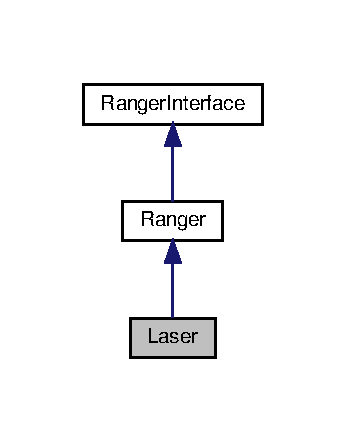
\includegraphics[width=166pt]{classLaser__inherit__graph}
\end{center}
\end{figure}


Collaboration diagram for Laser\+:\nopagebreak
\begin{figure}[H]
\begin{center}
\leavevmode
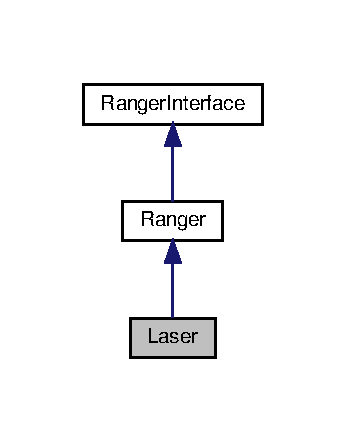
\includegraphics[width=166pt]{classLaser__coll__graph}
\end{center}
\end{figure}
\subsection*{Public Member Functions}
\begin{DoxyCompactItemize}
\item 
\hyperlink{classLaser_a68465e89283dffcc29a37e94693c6f87}{Laser} ()
\begin{DoxyCompactList}\small\item\em \hyperlink{classLaser}{Laser} default. \end{DoxyCompactList}\item 
\hyperlink{classLaser_abb99761eebf2ed73ab2fe3333c69dcdf}{Laser} (\hyperlink{structranger_1_1SensorPose}{ranger\+::\+Sensor\+Pose} pose)
\begin{DoxyCompactList}\small\item\em Costructor which would set defaults variables except position. \end{DoxyCompactList}\item 
\hyperlink{classLaser_a59ac47c673627b4af3fe3cc482545e1e}{Laser} (double maxr, double minr, unsigned int a\+Res, unsigned int fov, \hyperlink{structranger_1_1SensorPose}{ranger\+::\+Sensor\+Pose} pose, \hyperlink{namespacelaser_a986280215cdbdd42579d301afef1d22a}{laser\+::description} model)
\begin{DoxyCompactList}\small\item\em Costructor which would set all the variables of the sensor. \end{DoxyCompactList}\item 
std\+::vector$<$ double $>$ \hyperlink{classLaser_af2d93a5e123f3b637be6d3383019562b}{generate\+Data} ()
\begin{DoxyCompactList}\small\item\em Generates raw data for the sensor. \end{DoxyCompactList}\item 
bool \hyperlink{classLaser_a518ac84d4631b1550330d664e161ca0a}{set\+Angular\+Resolution} (unsigned int resolution)
\begin{DoxyCompactList}\small\item\em Sets the agular resolution of the sensor based on the model. \end{DoxyCompactList}\item 
bool \hyperlink{classLaser_a5f140784aae7e82c2aa0f690548d6ebb}{set\+Field\+Of\+View} (unsigned int fov)
\begin{DoxyCompactList}\small\item\em Sets the field of view (F\+OV) of the sensor based on the model. \end{DoxyCompactList}\end{DoxyCompactItemize}
\subsection*{Additional Inherited Members}


\subsection{Detailed Description}
The \hyperlink{classLaser}{Laser} type sensor class This class is derived from the base class \hyperlink{classRanger}{Ranger}. 

Used for \hyperlink{classLaser}{Laser} sensor creation. \hyperlink{classLaser}{Laser} returns Nl, number of measurements, distances, which are related to the specified angular resolution. Each measurements in a single point in space. The laser scans anticlockwise. 

\subsection{Constructor \& Destructor Documentation}
\mbox{\Hypertarget{classLaser_a68465e89283dffcc29a37e94693c6f87}\label{classLaser_a68465e89283dffcc29a37e94693c6f87}} 
\index{Laser@{Laser}!Laser@{Laser}}
\index{Laser@{Laser}!Laser@{Laser}}
\subsubsection{\texorpdfstring{Laser()}{Laser()}\hspace{0.1cm}{\footnotesize\ttfamily [1/3]}}
{\footnotesize\ttfamily Laser\+::\+Laser (\begin{DoxyParamCaption}{ }\end{DoxyParamCaption})}



\hyperlink{classLaser}{Laser} default. 

max range\+: 8 min range\+: 0.\+2 angular resolution\+: 10 fov\+: 180 position\+: 0,0,0 model\+:S\+I\+C\+K-\/\+XL \mbox{\Hypertarget{classLaser_abb99761eebf2ed73ab2fe3333c69dcdf}\label{classLaser_abb99761eebf2ed73ab2fe3333c69dcdf}} 
\index{Laser@{Laser}!Laser@{Laser}}
\index{Laser@{Laser}!Laser@{Laser}}
\subsubsection{\texorpdfstring{Laser()}{Laser()}\hspace{0.1cm}{\footnotesize\ttfamily [2/3]}}
{\footnotesize\ttfamily Laser\+::\+Laser (\begin{DoxyParamCaption}\item[{\hyperlink{structranger_1_1SensorPose}{ranger\+::\+Sensor\+Pose}}]{pose }\end{DoxyParamCaption})}



Costructor which would set defaults variables except position. 


\begin{DoxyParams}{Parameters}
{\em pose} & position \{x,y,theta\} \\
\hline
\end{DoxyParams}
\mbox{\Hypertarget{classLaser_a59ac47c673627b4af3fe3cc482545e1e}\label{classLaser_a59ac47c673627b4af3fe3cc482545e1e}} 
\index{Laser@{Laser}!Laser@{Laser}}
\index{Laser@{Laser}!Laser@{Laser}}
\subsubsection{\texorpdfstring{Laser()}{Laser()}\hspace{0.1cm}{\footnotesize\ttfamily [3/3]}}
{\footnotesize\ttfamily Laser\+::\+Laser (\begin{DoxyParamCaption}\item[{double}]{maxr,  }\item[{double}]{minr,  }\item[{unsigned int}]{a\+Res,  }\item[{unsigned int}]{fov,  }\item[{\hyperlink{structranger_1_1SensorPose}{ranger\+::\+Sensor\+Pose}}]{pose,  }\item[{\hyperlink{namespacelaser_a986280215cdbdd42579d301afef1d22a}{laser\+::description}}]{model }\end{DoxyParamCaption})}



Costructor which would set all the variables of the sensor. 


\begin{DoxyParams}{Parameters}
{\em maximum} & range \\
\hline
{\em minimum} & range \\
\hline
{\em angular} & resolution \\
\hline
{\em F\+OV} & -\/ angle \mbox{[}deg\mbox{]} \\
\hline
{\em position} & x \mbox{[}m\mbox{]}, y \mbox{[}m\mbox{]}, angle \mbox{[}radians\mbox{]} \\
\hline
\end{DoxyParams}


\subsection{Member Function Documentation}
\mbox{\Hypertarget{classLaser_af2d93a5e123f3b637be6d3383019562b}\label{classLaser_af2d93a5e123f3b637be6d3383019562b}} 
\index{Laser@{Laser}!generate\+Data@{generate\+Data}}
\index{generate\+Data@{generate\+Data}!Laser@{Laser}}
\subsubsection{\texorpdfstring{generate\+Data()}{generateData()}}
{\footnotesize\ttfamily std\+::vector$<$ double $>$ Laser\+::generate\+Data (\begin{DoxyParamCaption}{ }\end{DoxyParamCaption})\hspace{0.3cm}{\ttfamily [virtual]}}



Generates raw data for the sensor. 

\begin{DoxyReturn}{Returns}
vector containing senor data
\end{DoxyReturn}
returning vector of doubles contain \textquotesingle{}Nl\textquotesingle{} number of reading. \textquotesingle{}Nl\textquotesingle{} is an integer number of readings (F\+O\+V/angular resolution)+1. The values should be distances to points within the F\+OV range between min and max range.

The function calculates Nl number of distances, between min and max. 

Implements \hyperlink{classRanger_a1ac4a84f251b0793fc262643080f084a}{Ranger}.

\mbox{\Hypertarget{classLaser_a518ac84d4631b1550330d664e161ca0a}\label{classLaser_a518ac84d4631b1550330d664e161ca0a}} 
\index{Laser@{Laser}!set\+Angular\+Resolution@{set\+Angular\+Resolution}}
\index{set\+Angular\+Resolution@{set\+Angular\+Resolution}!Laser@{Laser}}
\subsubsection{\texorpdfstring{set\+Angular\+Resolution()}{setAngularResolution()}}
{\footnotesize\ttfamily bool Laser\+::set\+Angular\+Resolution (\begin{DoxyParamCaption}\item[{unsigned int}]{resolution }\end{DoxyParamCaption})\hspace{0.3cm}{\ttfamily [virtual]}}



Sets the agular resolution of the sensor based on the model. 


\begin{DoxyParams}{Parameters}
{\em resolution} & \mbox{[}deg\mbox{]} \\
\hline
\end{DoxyParams}
\begin{DoxyReturn}{Returns}
True if supported and actioned, false otherwise.
\end{DoxyReturn}
Actioned if the value is acceptable based on the model of the laser. (10 or 30 for S\+I\+C\+K-\/\+XL) 

Reimplemented from \hyperlink{classRanger_a3dc62dcba54eefbd7a0f08cbf97d87dc}{Ranger}.

\mbox{\Hypertarget{classLaser_a5f140784aae7e82c2aa0f690548d6ebb}\label{classLaser_a5f140784aae7e82c2aa0f690548d6ebb}} 
\index{Laser@{Laser}!set\+Field\+Of\+View@{set\+Field\+Of\+View}}
\index{set\+Field\+Of\+View@{set\+Field\+Of\+View}!Laser@{Laser}}
\subsubsection{\texorpdfstring{set\+Field\+Of\+View()}{setFieldOfView()}}
{\footnotesize\ttfamily bool Laser\+::set\+Field\+Of\+View (\begin{DoxyParamCaption}\item[{unsigned int}]{fov }\end{DoxyParamCaption})\hspace{0.3cm}{\ttfamily [virtual]}}



Sets the field of view (F\+OV) of the sensor based on the model. 


\begin{DoxyParams}{Parameters}
{\em F\+OV} & value \mbox{[}deg\mbox{]} \\
\hline
\end{DoxyParams}
\begin{DoxyReturn}{Returns}
True if actioned, false otherwise
\end{DoxyReturn}
F\+OV would be a value between 0 and 360 degrees for the command to be actioned (only 180 for S\+I\+C\+K-\/\+XL, connot be changed for this model) 

Reimplemented from \hyperlink{classRanger_afb5d392ca450bcce295e61c121d09157}{Ranger}.



The documentation for this class was generated from the following files\+:\begin{DoxyCompactItemize}
\item 
laser.\+h\item 
laser.\+cpp\end{DoxyCompactItemize}

\hypertarget{classLine}{}\section{Line Class Reference}
\label{classLine}\index{Line@{Line}}


\hyperlink{classLine}{Line} class.  




{\ttfamily \#include $<$line.\+h$>$}

\subsection*{Public Member Functions}
\begin{DoxyCompactItemize}
\item 
\hyperlink{classLine_abad81a289f4a192ebdfdaae35dcd8a87}{Line} (\hyperlink{structgeometry__msgs_1_1Point}{geometry\+\_\+msgs\+::\+Point} pt1, \hyperlink{structgeometry__msgs_1_1Point}{geometry\+\_\+msgs\+::\+Point} pt2)
\begin{DoxyCompactList}\small\item\em Default constructor. \end{DoxyCompactList}\item 
bool \hyperlink{classLine_a058bf81f941f204ec351925660c296b3}{point\+Above\+Line} (\hyperlink{structgeometry__msgs_1_1Point}{geometry\+\_\+msgs\+::\+Point} pt)
\begin{DoxyCompactList}\small\item\em checks if a point is above the \hyperlink{classLine}{Line} \end{DoxyCompactList}\item 
double \hyperlink{classLine_a872b756c94ed478d05e430ebb436b116}{get\+Gradient} ()
\begin{DoxyCompactList}\small\item\em gets the Gradient \end{DoxyCompactList}\item 
double \hyperlink{classLine_ac3bf0f79e9748a26ad1dd347fe97da75}{get\+Y\+Intercept} ()
\begin{DoxyCompactList}\small\item\em gets the Y-\/\+Intercept \end{DoxyCompactList}\item 
void \hyperlink{classLine_acc07117e5463e70ee1159b55d5dc4502}{get\+Points} (\hyperlink{structgeometry__msgs_1_1Point}{geometry\+\_\+msgs\+::\+Point} \&pt1, \hyperlink{structgeometry__msgs_1_1Point}{geometry\+\_\+msgs\+::\+Point} \&pt2)
\begin{DoxyCompactList}\small\item\em get the two Points of the line segment \end{DoxyCompactList}\end{DoxyCompactItemize}


\subsection{Detailed Description}
\hyperlink{classLine}{Line} class. 

Creates a \hyperlink{classLine}{Line} between given points in space, and stores its geometric properties \begin{DoxyAuthor}{Author}
Chamath Edirisinhege 
\end{DoxyAuthor}
\begin{DoxyVersion}{Version}
1.\+0 
\end{DoxyVersion}
\begin{DoxyDate}{Date}
2021-\/08-\/31 
\end{DoxyDate}
\begin{DoxyRefDesc}{Bug}
\item[\hyperlink{bug__bug000004}{Bug}]none reported as of 2021-\/09-\/07 \end{DoxyRefDesc}


Lreates a line, and stores its geometric properties. Taken from quiz2 and then modified. 

\subsection{Constructor \& Destructor Documentation}
\mbox{\Hypertarget{classLine_abad81a289f4a192ebdfdaae35dcd8a87}\label{classLine_abad81a289f4a192ebdfdaae35dcd8a87}} 
\index{Line@{Line}!Line@{Line}}
\index{Line@{Line}!Line@{Line}}
\subsubsection{\texorpdfstring{Line()}{Line()}}
{\footnotesize\ttfamily Line\+::\+Line (\begin{DoxyParamCaption}\item[{\hyperlink{structgeometry__msgs_1_1Point}{geometry\+\_\+msgs\+::\+Point}}]{pt1,  }\item[{\hyperlink{structgeometry__msgs_1_1Point}{geometry\+\_\+msgs\+::\+Point}}]{pt2 }\end{DoxyParamCaption})}



Default constructor. 


\begin{DoxyParams}{Parameters}
{\em starting} & point, ending point\\
\hline
\end{DoxyParams}
generates a line segment between the two points. 

\subsection{Member Function Documentation}
\mbox{\Hypertarget{classLine_a872b756c94ed478d05e430ebb436b116}\label{classLine_a872b756c94ed478d05e430ebb436b116}} 
\index{Line@{Line}!get\+Gradient@{get\+Gradient}}
\index{get\+Gradient@{get\+Gradient}!Line@{Line}}
\subsubsection{\texorpdfstring{get\+Gradient()}{getGradient()}}
{\footnotesize\ttfamily double Line\+::get\+Gradient (\begin{DoxyParamCaption}{ }\end{DoxyParamCaption})}



gets the Gradient 

\begin{DoxyReturn}{Returns}
gradient 
\end{DoxyReturn}
\mbox{\Hypertarget{classLine_acc07117e5463e70ee1159b55d5dc4502}\label{classLine_acc07117e5463e70ee1159b55d5dc4502}} 
\index{Line@{Line}!get\+Points@{get\+Points}}
\index{get\+Points@{get\+Points}!Line@{Line}}
\subsubsection{\texorpdfstring{get\+Points()}{getPoints()}}
{\footnotesize\ttfamily void Line\+::get\+Points (\begin{DoxyParamCaption}\item[{\hyperlink{structgeometry__msgs_1_1Point}{geometry\+\_\+msgs\+::\+Point} \&}]{pt1,  }\item[{\hyperlink{structgeometry__msgs_1_1Point}{geometry\+\_\+msgs\+::\+Point} \&}]{pt2 }\end{DoxyParamCaption})}



get the two Points of the line segment 


\begin{DoxyParams}{Parameters}
{\em pt1} & holding variable for first point \\
\hline
{\em pt2} & holding variable for first point \\
\hline
\end{DoxyParams}
\mbox{\Hypertarget{classLine_ac3bf0f79e9748a26ad1dd347fe97da75}\label{classLine_ac3bf0f79e9748a26ad1dd347fe97da75}} 
\index{Line@{Line}!get\+Y\+Intercept@{get\+Y\+Intercept}}
\index{get\+Y\+Intercept@{get\+Y\+Intercept}!Line@{Line}}
\subsubsection{\texorpdfstring{get\+Y\+Intercept()}{getYIntercept()}}
{\footnotesize\ttfamily double Line\+::get\+Y\+Intercept (\begin{DoxyParamCaption}{ }\end{DoxyParamCaption})}



gets the Y-\/\+Intercept 

\begin{DoxyReturn}{Returns}
y intercept 
\end{DoxyReturn}
\mbox{\Hypertarget{classLine_a058bf81f941f204ec351925660c296b3}\label{classLine_a058bf81f941f204ec351925660c296b3}} 
\index{Line@{Line}!point\+Above\+Line@{point\+Above\+Line}}
\index{point\+Above\+Line@{point\+Above\+Line}!Line@{Line}}
\subsubsection{\texorpdfstring{point\+Above\+Line()}{pointAboveLine()}}
{\footnotesize\ttfamily bool Line\+::point\+Above\+Line (\begin{DoxyParamCaption}\item[{\hyperlink{structgeometry__msgs_1_1Point}{geometry\+\_\+msgs\+::\+Point}}]{pt }\end{DoxyParamCaption})}



checks if a point is above the \hyperlink{classLine}{Line} 


\begin{DoxyParams}{Parameters}
{\em pt} & -\/ test point \\
\hline
\end{DoxyParams}
\begin{DoxyReturn}{Returns}
true if test point is above the line 
\end{DoxyReturn}


The documentation for this class was generated from the following files\+:\begin{DoxyCompactItemize}
\item 
line.\+h\item 
line.\+cpp\end{DoxyCompactItemize}

\hypertarget{structgeometry__msgs_1_1Point}{}\section{geometry\+\_\+msgs\+:\+:Point Struct Reference}
\label{structgeometry__msgs_1_1Point}\index{geometry\+\_\+msgs\+::\+Point@{geometry\+\_\+msgs\+::\+Point}}


{\ttfamily \#include $<$line.\+h$>$}

\subsection*{Public Attributes}
\begin{DoxyCompactItemize}
\item 
\mbox{\Hypertarget{structgeometry__msgs_1_1Point_a52ccd2ddf703b661ed049c2a41e1525f}\label{structgeometry__msgs_1_1Point_a52ccd2ddf703b661ed049c2a41e1525f}} 
double \hyperlink{structgeometry__msgs_1_1Point_a52ccd2ddf703b661ed049c2a41e1525f}{x}
\begin{DoxyCompactList}\small\item\em x position \end{DoxyCompactList}\item 
\mbox{\Hypertarget{structgeometry__msgs_1_1Point_a8b028e43156db47fed28583d9b196d89}\label{structgeometry__msgs_1_1Point_a8b028e43156db47fed28583d9b196d89}} 
double \hyperlink{structgeometry__msgs_1_1Point_a8b028e43156db47fed28583d9b196d89}{y}
\begin{DoxyCompactList}\small\item\em y position \end{DoxyCompactList}\end{DoxyCompactItemize}


\subsection{Detailed Description}
Structure for 2d Positions 

The documentation for this struct was generated from the following file\+:\begin{DoxyCompactItemize}
\item 
line.\+h\end{DoxyCompactItemize}

\hypertarget{classRanger}{}\section{Ranger Class Reference}
\label{classRanger}\index{Ranger@{Ranger}}


\hyperlink{classRanger}{Ranger} base Class.  




{\ttfamily \#include $<$ranger.\+h$>$}



Inheritance diagram for Ranger\+:\nopagebreak
\begin{figure}[H]
\begin{center}
\leavevmode
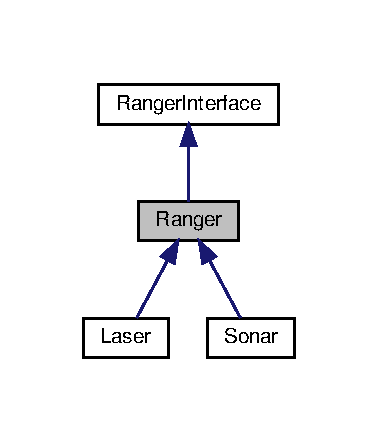
\includegraphics[width=182pt]{classRanger__inherit__graph}
\end{center}
\end{figure}


Collaboration diagram for Ranger\+:\nopagebreak
\begin{figure}[H]
\begin{center}
\leavevmode
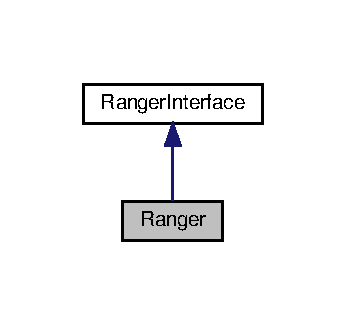
\includegraphics[width=166pt]{classRanger__coll__graph}
\end{center}
\end{figure}
\subsection*{Public Member Functions}
\begin{DoxyCompactItemize}
\item 
\hyperlink{classRanger_ad87e3ddf656eae8f77c88297a313c8a1}{Ranger} (double maxr, double minr, unsigned int a\+Res, unsigned int fov, \hyperlink{structranger_1_1SensorPose}{ranger\+::\+Sensor\+Pose} pose, \hyperlink{namespaceranger_ab04465c229cc50595ffe40a891a3b135}{ranger\+::\+Sensing\+Method} method)
\begin{DoxyCompactList}\small\item\em Costructor which would set all the variables of the sensor. \end{DoxyCompactList}\item 
virtual std\+::vector$<$ double $>$ \hyperlink{classRanger_a1ac4a84f251b0793fc262643080f084a}{generate\+Data} ()=0
\begin{DoxyCompactList}\small\item\em \hyperlink{classRanger}{Ranger} is an abstract class and requires a virtual destructor. \end{DoxyCompactList}\item 
unsigned int \hyperlink{classRanger_a95b5013ae191d1e19b93fab002306718}{get\+Angular\+Resolution} (void)
\begin{DoxyCompactList}\small\item\em Gets the angular resolution. \end{DoxyCompactList}\item 
\hyperlink{structranger_1_1SensorPose}{ranger\+::\+Sensor\+Pose} \hyperlink{classRanger_aec1e730fbf4b46b01b08f6655152fc39}{get\+Sensor\+Pose} (void)
\begin{DoxyCompactList}\small\item\em Gets the sensor position information. \end{DoxyCompactList}\item 
unsigned int \hyperlink{classRanger_a4bca7dce56b7959257d90b1f30bf0271}{get\+Field\+Of\+View} (void)
\begin{DoxyCompactList}\small\item\em Gets sensor field of view (F\+OV). F\+OV of point based sensors, is zero. \end{DoxyCompactList}\item 
double \hyperlink{classRanger_aba5e81260e55089d9ff869051156a722}{get\+Max\+Range} (void)
\begin{DoxyCompactList}\small\item\em Gets the maximum range of the sensor. \end{DoxyCompactList}\item 
double \hyperlink{classRanger_a646a06d3916179b9ebc4502bad169eec}{get\+Min\+Range} (void)
\begin{DoxyCompactList}\small\item\em Gets the minimum range of the sensor. \end{DoxyCompactList}\item 
\hyperlink{namespaceranger_ab04465c229cc50595ffe40a891a3b135}{ranger\+::\+Sensing\+Method} \hyperlink{classRanger_a47e30b7ec55adec5bb542278ccfee140}{get\+Sensing\+Method} (void)
\begin{DoxyCompactList}\small\item\em Gets the sensing method. \end{DoxyCompactList}\item 
virtual bool \hyperlink{classRanger_a3dc62dcba54eefbd7a0f08cbf97d87dc}{set\+Angular\+Resolution} (unsigned int resolution)
\begin{DoxyCompactList}\small\item\em Sets the agular resolution of the sensor. \end{DoxyCompactList}\item 
bool \hyperlink{classRanger_aa55ad45d83b8c095a495677ac8873f2b}{set\+Sensor\+Pose} (\hyperlink{structranger_1_1SensorPose}{ranger\+::\+Sensor\+Pose} pose)
\begin{DoxyCompactList}\small\item\em Sets an offset to the original position and angle of the sensor. \end{DoxyCompactList}\item 
virtual bool \hyperlink{classRanger_afb5d392ca450bcce295e61c121d09157}{set\+Field\+Of\+View} (unsigned int fov)
\begin{DoxyCompactList}\small\item\em Sets the field of view (F\+OV) of the sensor. \end{DoxyCompactList}\item 
double \hyperlink{classRanger_a35dfc3ff4e5c6c31a8625e972365006e}{get\+Sequence\+Num} ()
\begin{DoxyCompactList}\small\item\em Gets the number of readings taken by the sensor. \end{DoxyCompactList}\end{DoxyCompactItemize}
\subsection*{Protected Attributes}
\begin{DoxyCompactItemize}
\item 
\mbox{\Hypertarget{classRanger_aa92901df85f1818f27c0cf2e56ac2667}\label{classRanger_aa92901df85f1818f27c0cf2e56ac2667}} 
double {\bfseries max\+Range\+\_\+}
\item 
\mbox{\Hypertarget{classRanger_a3dddeb9eb109baf567dfcd356706c6fb}\label{classRanger_a3dddeb9eb109baf567dfcd356706c6fb}} 
double \hyperlink{classRanger_a3dddeb9eb109baf567dfcd356706c6fb}{min\+Range\+\_\+}
\begin{DoxyCompactList}\small\item\em maximum range of the sensor \end{DoxyCompactList}\item 
\mbox{\Hypertarget{classRanger_acc6c665b0e64c74c837753aba184b19d}\label{classRanger_acc6c665b0e64c74c837753aba184b19d}} 
unsigned int \hyperlink{classRanger_acc6c665b0e64c74c837753aba184b19d}{F\+O\+V\+\_\+}
\begin{DoxyCompactList}\small\item\em minimum range of the sensor \end{DoxyCompactList}\item 
\mbox{\Hypertarget{classRanger_abf27486783526e849e3752036ea16ba7}\label{classRanger_abf27486783526e849e3752036ea16ba7}} 
unsigned int \hyperlink{classRanger_abf27486783526e849e3752036ea16ba7}{ang\+Resolution\+\_\+} = 0
\begin{DoxyCompactList}\small\item\em field of view of the sensor \end{DoxyCompactList}\item 
\mbox{\Hypertarget{classRanger_ae7402070c4b7ad80b2ab0af7e1dfc3b0}\label{classRanger_ae7402070c4b7ad80b2ab0af7e1dfc3b0}} 
unsigned int \hyperlink{classRanger_ae7402070c4b7ad80b2ab0af7e1dfc3b0}{sequence\+Num\+\_\+} = 0
\begin{DoxyCompactList}\small\item\em angular resolution of the sensor \end{DoxyCompactList}\end{DoxyCompactItemize}


\subsection{Detailed Description}
\hyperlink{classRanger}{Ranger} base Class. 

The \hyperlink{classRanger}{Ranger} Fusion class. This class is derived from the interface class ranger fusion interface.

This base class is used to set all the methods that need to be embodied within any subsequent derived sensor classes. Contains all the setters and getters for sensor variables. \begin{DoxyAuthor}{Author}
Chamath Edirisinhege 
\end{DoxyAuthor}
\begin{DoxyVersion}{Version}
1.\+0 
\end{DoxyVersion}
\begin{DoxyDate}{Date}
2021-\/08-\/31 
\end{DoxyDate}
\begin{DoxyRefDesc}{Bug}
\item[\hyperlink{bug__bug000006}{Bug}]none reported as of 2021-\/09-\/07 \end{DoxyRefDesc}


The \hyperlink{classRanger}{Ranger} base class for sensors. This class is derived from the interface class ranger interface

Used for sensor creation

Accept a container of Sensors and a container of Cells. Then determine the area convered by the sensors as a whole. Produce sensor readings and then checks for interaction with cells and label the cells accordingly. This class uses the geometry library and its classes for calculations. 

\subsection{Constructor \& Destructor Documentation}
\mbox{\Hypertarget{classRanger_ad87e3ddf656eae8f77c88297a313c8a1}\label{classRanger_ad87e3ddf656eae8f77c88297a313c8a1}} 
\index{Ranger@{Ranger}!Ranger@{Ranger}}
\index{Ranger@{Ranger}!Ranger@{Ranger}}
\subsubsection{\texorpdfstring{Ranger()}{Ranger()}}
{\footnotesize\ttfamily Ranger\+::\+Ranger (\begin{DoxyParamCaption}\item[{double}]{maxr,  }\item[{double}]{minr,  }\item[{unsigned int}]{a\+Res,  }\item[{unsigned int}]{fov,  }\item[{\hyperlink{structranger_1_1SensorPose}{ranger\+::\+Sensor\+Pose}}]{pose,  }\item[{\hyperlink{namespaceranger_ab04465c229cc50595ffe40a891a3b135}{ranger\+::\+Sensing\+Method}}]{method }\end{DoxyParamCaption})}



Costructor which would set all the variables of the sensor. 


\begin{DoxyParams}{Parameters}
{\em maximum} & range \\
\hline
{\em minimum} & range \\
\hline
{\em angular} & resolution \\
\hline
{\em F\+OV} & -\/ angle \mbox{[}deg\mbox{]} \\
\hline
{\em position} & x \mbox{[}m\mbox{]}, y \mbox{[}m\mbox{]}, angle \mbox{[}radians\mbox{]} \\
\hline
{\em Sensing} & method\+: cone or point? \\
\hline
\end{DoxyParams}


\subsection{Member Function Documentation}
\mbox{\Hypertarget{classRanger_a1ac4a84f251b0793fc262643080f084a}\label{classRanger_a1ac4a84f251b0793fc262643080f084a}} 
\index{Ranger@{Ranger}!generate\+Data@{generate\+Data}}
\index{generate\+Data@{generate\+Data}!Ranger@{Ranger}}
\subsubsection{\texorpdfstring{generate\+Data()}{generateData()}}
{\footnotesize\ttfamily virtual std\+::vector$<$double$>$ Ranger\+::generate\+Data (\begin{DoxyParamCaption}{ }\end{DoxyParamCaption})\hspace{0.3cm}{\ttfamily [pure virtual]}}



\hyperlink{classRanger}{Ranger} is an abstract class and requires a virtual destructor. 

generate raw Data \begin{DoxyReturn}{Returns}
vector of data points 
\end{DoxyReturn}


Implements \hyperlink{classRangerInterface}{Ranger\+Interface}.



Implemented in \hyperlink{classLaser_af2d93a5e123f3b637be6d3383019562b}{Laser}, and \hyperlink{classSonar_a33cc5f2df6cc1d96a59067be67eab781}{Sonar}.

\mbox{\Hypertarget{classRanger_a95b5013ae191d1e19b93fab002306718}\label{classRanger_a95b5013ae191d1e19b93fab002306718}} 
\index{Ranger@{Ranger}!get\+Angular\+Resolution@{get\+Angular\+Resolution}}
\index{get\+Angular\+Resolution@{get\+Angular\+Resolution}!Ranger@{Ranger}}
\subsubsection{\texorpdfstring{get\+Angular\+Resolution()}{getAngularResolution()}}
{\footnotesize\ttfamily unsigned int Ranger\+::get\+Angular\+Resolution (\begin{DoxyParamCaption}\item[{void}]{ }\end{DoxyParamCaption})\hspace{0.3cm}{\ttfamily [virtual]}}



Gets the angular resolution. 

\begin{DoxyReturn}{Returns}
angular resolution of the sensor 
\end{DoxyReturn}


Implements \hyperlink{classRangerInterface_a37d4f89daffa8b2708dfc11034893552}{Ranger\+Interface}.

\mbox{\Hypertarget{classRanger_a4bca7dce56b7959257d90b1f30bf0271}\label{classRanger_a4bca7dce56b7959257d90b1f30bf0271}} 
\index{Ranger@{Ranger}!get\+Field\+Of\+View@{get\+Field\+Of\+View}}
\index{get\+Field\+Of\+View@{get\+Field\+Of\+View}!Ranger@{Ranger}}
\subsubsection{\texorpdfstring{get\+Field\+Of\+View()}{getFieldOfView()}}
{\footnotesize\ttfamily unsigned int Ranger\+::get\+Field\+Of\+View (\begin{DoxyParamCaption}\item[{void}]{ }\end{DoxyParamCaption})\hspace{0.3cm}{\ttfamily [virtual]}}



Gets sensor field of view (F\+OV). F\+OV of point based sensors, is zero. 

\begin{DoxyReturn}{Returns}
the F\+OV angle \mbox{[}deg\mbox{]} 
\end{DoxyReturn}


Implements \hyperlink{classRangerInterface_a18716da6932402b8dda75f682be6f06c}{Ranger\+Interface}.

\mbox{\Hypertarget{classRanger_aba5e81260e55089d9ff869051156a722}\label{classRanger_aba5e81260e55089d9ff869051156a722}} 
\index{Ranger@{Ranger}!get\+Max\+Range@{get\+Max\+Range}}
\index{get\+Max\+Range@{get\+Max\+Range}!Ranger@{Ranger}}
\subsubsection{\texorpdfstring{get\+Max\+Range()}{getMaxRange()}}
{\footnotesize\ttfamily double Ranger\+::get\+Max\+Range (\begin{DoxyParamCaption}\item[{void}]{ }\end{DoxyParamCaption})\hspace{0.3cm}{\ttfamily [virtual]}}



Gets the maximum range of the sensor. 

\begin{DoxyReturn}{Returns}
maximum range \mbox{[}m\mbox{]} 
\end{DoxyReturn}


Implements \hyperlink{classRangerInterface_a0bb29a41de5767c99081002c0590c186}{Ranger\+Interface}.

\mbox{\Hypertarget{classRanger_a646a06d3916179b9ebc4502bad169eec}\label{classRanger_a646a06d3916179b9ebc4502bad169eec}} 
\index{Ranger@{Ranger}!get\+Min\+Range@{get\+Min\+Range}}
\index{get\+Min\+Range@{get\+Min\+Range}!Ranger@{Ranger}}
\subsubsection{\texorpdfstring{get\+Min\+Range()}{getMinRange()}}
{\footnotesize\ttfamily double Ranger\+::get\+Min\+Range (\begin{DoxyParamCaption}\item[{void}]{ }\end{DoxyParamCaption})\hspace{0.3cm}{\ttfamily [virtual]}}



Gets the minimum range of the sensor. 

\begin{DoxyReturn}{Returns}
minimum range \mbox{[}m\mbox{]} 
\end{DoxyReturn}


Implements \hyperlink{classRangerInterface_ae6d501ddeeaad4a7b44d7d51ce64cb88}{Ranger\+Interface}.

\mbox{\Hypertarget{classRanger_a47e30b7ec55adec5bb542278ccfee140}\label{classRanger_a47e30b7ec55adec5bb542278ccfee140}} 
\index{Ranger@{Ranger}!get\+Sensing\+Method@{get\+Sensing\+Method}}
\index{get\+Sensing\+Method@{get\+Sensing\+Method}!Ranger@{Ranger}}
\subsubsection{\texorpdfstring{get\+Sensing\+Method()}{getSensingMethod()}}
{\footnotesize\ttfamily \hyperlink{namespaceranger_ab04465c229cc50595ffe40a891a3b135}{ranger\+::\+Sensing\+Method} Ranger\+::get\+Sensing\+Method (\begin{DoxyParamCaption}\item[{void}]{ }\end{DoxyParamCaption})\hspace{0.3cm}{\ttfamily [virtual]}}



Gets the sensing method. 

\begin{DoxyReturn}{Returns}
sensing method 
\end{DoxyReturn}


Implements \hyperlink{classRangerInterface_aeb06b9835f2b162b81917bd27797549b}{Ranger\+Interface}.

\mbox{\Hypertarget{classRanger_aec1e730fbf4b46b01b08f6655152fc39}\label{classRanger_aec1e730fbf4b46b01b08f6655152fc39}} 
\index{Ranger@{Ranger}!get\+Sensor\+Pose@{get\+Sensor\+Pose}}
\index{get\+Sensor\+Pose@{get\+Sensor\+Pose}!Ranger@{Ranger}}
\subsubsection{\texorpdfstring{get\+Sensor\+Pose()}{getSensorPose()}}
{\footnotesize\ttfamily \hyperlink{structranger_1_1SensorPose}{ranger\+::\+Sensor\+Pose} Ranger\+::get\+Sensor\+Pose (\begin{DoxyParamCaption}\item[{void}]{ }\end{DoxyParamCaption})\hspace{0.3cm}{\ttfamily [virtual]}}



Gets the sensor position information. 

\begin{DoxyReturn}{Returns}
x \mbox{[}m\mbox{]}, y \mbox{[}m\mbox{]} position coordinate and angle \mbox{[}radians\mbox{]} 
\end{DoxyReturn}


Implements \hyperlink{classRangerInterface_a7f6db3f603d997ad6c5aa5c7778261f4}{Ranger\+Interface}.

\mbox{\Hypertarget{classRanger_a35dfc3ff4e5c6c31a8625e972365006e}\label{classRanger_a35dfc3ff4e5c6c31a8625e972365006e}} 
\index{Ranger@{Ranger}!get\+Sequence\+Num@{get\+Sequence\+Num}}
\index{get\+Sequence\+Num@{get\+Sequence\+Num}!Ranger@{Ranger}}
\subsubsection{\texorpdfstring{get\+Sequence\+Num()}{getSequenceNum()}}
{\footnotesize\ttfamily double Ranger\+::get\+Sequence\+Num (\begin{DoxyParamCaption}{ }\end{DoxyParamCaption})}



Gets the number of readings taken by the sensor. 

\begin{DoxyReturn}{Returns}
number of readings taken by the sensor 
\end{DoxyReturn}
\mbox{\Hypertarget{classRanger_a3dc62dcba54eefbd7a0f08cbf97d87dc}\label{classRanger_a3dc62dcba54eefbd7a0f08cbf97d87dc}} 
\index{Ranger@{Ranger}!set\+Angular\+Resolution@{set\+Angular\+Resolution}}
\index{set\+Angular\+Resolution@{set\+Angular\+Resolution}!Ranger@{Ranger}}
\subsubsection{\texorpdfstring{set\+Angular\+Resolution()}{setAngularResolution()}}
{\footnotesize\ttfamily bool Ranger\+::set\+Angular\+Resolution (\begin{DoxyParamCaption}\item[{unsigned int}]{resolution }\end{DoxyParamCaption})\hspace{0.3cm}{\ttfamily [virtual]}}



Sets the agular resolution of the sensor. 


\begin{DoxyParams}{Parameters}
{\em resolution} & \mbox{[}deg\mbox{]} \\
\hline
\end{DoxyParams}
\begin{DoxyReturn}{Returns}
True if supported and actioned, false otherwise.
\end{DoxyReturn}
As the default it will be actioned and always true. Defines the angular \textquotesingle{}gap\textquotesingle{} between two consecutive readings. Must be between 0 and F\+OV. 

Implements \hyperlink{classRangerInterface_aecffc9bbb58379da741c18326b9e41db}{Ranger\+Interface}.



Reimplemented in \hyperlink{classLaser_a518ac84d4631b1550330d664e161ca0a}{Laser}.

\mbox{\Hypertarget{classRanger_afb5d392ca450bcce295e61c121d09157}\label{classRanger_afb5d392ca450bcce295e61c121d09157}} 
\index{Ranger@{Ranger}!set\+Field\+Of\+View@{set\+Field\+Of\+View}}
\index{set\+Field\+Of\+View@{set\+Field\+Of\+View}!Ranger@{Ranger}}
\subsubsection{\texorpdfstring{set\+Field\+Of\+View()}{setFieldOfView()}}
{\footnotesize\ttfamily bool Ranger\+::set\+Field\+Of\+View (\begin{DoxyParamCaption}\item[{unsigned int}]{fov }\end{DoxyParamCaption})\hspace{0.3cm}{\ttfamily [virtual]}}



Sets the field of view (F\+OV) of the sensor. 


\begin{DoxyParams}{Parameters}
{\em F\+OV} & value \mbox{[}deg\mbox{]} \\
\hline
\end{DoxyParams}
\begin{DoxyReturn}{Returns}
True if actioned, false otherwise
\end{DoxyReturn}
F\+OV would be a value between 0 and 360 degrees for the command to be actioned 

Implements \hyperlink{classRangerInterface_a70357ca516198af45e2d503ef6af8f9f}{Ranger\+Interface}.



Reimplemented in \hyperlink{classLaser_a5f140784aae7e82c2aa0f690548d6ebb}{Laser}, and \hyperlink{classSonar_a74d551d0ad61861ccf903f2535d799f0}{Sonar}.

\mbox{\Hypertarget{classRanger_aa55ad45d83b8c095a495677ac8873f2b}\label{classRanger_aa55ad45d83b8c095a495677ac8873f2b}} 
\index{Ranger@{Ranger}!set\+Sensor\+Pose@{set\+Sensor\+Pose}}
\index{set\+Sensor\+Pose@{set\+Sensor\+Pose}!Ranger@{Ranger}}
\subsubsection{\texorpdfstring{set\+Sensor\+Pose()}{setSensorPose()}}
{\footnotesize\ttfamily bool Ranger\+::set\+Sensor\+Pose (\begin{DoxyParamCaption}\item[{\hyperlink{structranger_1_1SensorPose}{ranger\+::\+Sensor\+Pose}}]{pose }\end{DoxyParamCaption})\hspace{0.3cm}{\ttfamily [virtual]}}



Sets an offset to the original position and angle of the sensor. 


\begin{DoxyParams}{Parameters}
{\em pose} & x position \mbox{[}m\mbox{]}, y position \mbox{[}m\mbox{]}, angle \mbox{[}radians\mbox{]} \\
\hline
\end{DoxyParams}
\begin{DoxyReturn}{Returns}
True if actioned, false otherwise
\end{DoxyReturn}
Theta value has to be between 2\+PI and 0, therefore when it has been off set by 2\+PI it has returned to it initial position. The if statement makes sure that theta would like between 0 and 2\+PI, by adding or substracting 2\+PI from theta when it goes past the respective boundries. 

Implements \hyperlink{classRangerInterface_a452301937b5ace7ded943d8aa76a061f}{Ranger\+Interface}.



The documentation for this class was generated from the following files\+:\begin{DoxyCompactItemize}
\item 
ranger.\+h\item 
ranger.\+cpp\end{DoxyCompactItemize}

\hypertarget{classRangerFusion}{}\section{Ranger\+Fusion Class Reference}
\label{classRangerFusion}\index{Ranger\+Fusion@{Ranger\+Fusion}}


Inheritance diagram for Ranger\+Fusion\+:\nopagebreak
\begin{figure}[H]
\begin{center}
\leavevmode
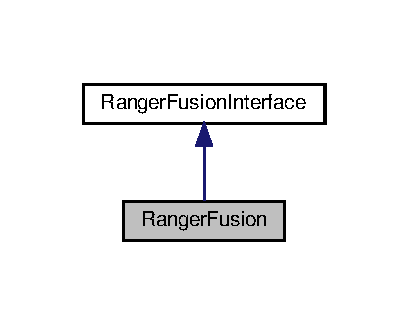
\includegraphics[width=196pt]{classRangerFusion__inherit__graph}
\end{center}
\end{figure}


Collaboration diagram for Ranger\+Fusion\+:\nopagebreak
\begin{figure}[H]
\begin{center}
\leavevmode
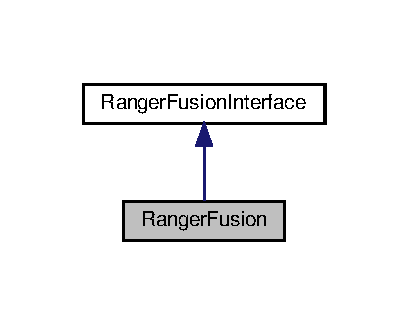
\includegraphics[width=196pt]{classRangerFusion__coll__graph}
\end{center}
\end{figure}
\subsection*{Public Member Functions}
\begin{DoxyCompactItemize}
\item 
\hyperlink{classRangerFusion_ae06d13fa52742f42e138b386e5022168}{Ranger\+Fusion} (std\+::vector$<$ \hyperlink{classRangerInterface}{Ranger\+Interface} $\ast$$>$ rangers)
\item 
void \hyperlink{classRangerFusion_aaf0f90048ff744580eeb73a2bf3a38f7}{get\+Cells} (std\+::vector$<$ \hyperlink{classCell}{Cell} $\ast$$>$ \&cells)
\begin{DoxyCompactList}\small\item\em Returns the container of cells. \end{DoxyCompactList}\item 
void \hyperlink{classRangerFusion_a9b69869bd1e3bca155bcecbad5ea463b}{set\+Cells} (std\+::vector$<$ \hyperlink{classCell}{Cell} $\ast$$>$ cells)
\begin{DoxyCompactList}\small\item\em Accepts the container of cells. \end{DoxyCompactList}\item 
\mbox{\Hypertarget{classRangerFusion_aa9265f72bc3572567c9cf98cf6d9f0e1}\label{classRangerFusion_aa9265f72bc3572567c9cf98cf6d9f0e1}} 
void \hyperlink{classRangerFusion_aa9265f72bc3572567c9cf98cf6d9f0e1}{grab\+And\+Fuse\+Data} ()
\begin{DoxyCompactList}\small\item\em Does two operations (1) Calls each ranger to generate data and uses this data to determine colissions with provided container of cells (2) Generates a \textquotesingle{}fusion\textquotesingle{} of the data based on collision conditions as descibed in Assignment 2 specification. \end{DoxyCompactList}\item 
std\+::vector$<$ std\+::vector$<$ double $>$ $>$ \hyperlink{classRangerFusion_a5780383fdffe121a7a2372a047819ba9}{get\+Raw\+Range\+Data} ()
\begin{DoxyCompactList}\small\item\em Returns the raw data from all sensors in the ranger container within a vector of vectors The raw data is updated every time a new fusion is requested (grab\+And\+Fuse\+Dat). The raw data is the data used for collision checking. If no fusion has occured the vector shall be empty. \end{DoxyCompactList}\item 
double \hyperlink{classRangerFusion_a7215e5405e808b5a853984e2b70ed6ad}{get\+Scanning\+Area} ()
\begin{DoxyCompactList}\small\item\em Returns the total scanning area possible with C\+O\+NE based scanners supplied A union of all areas \href{https://en.wikipedia.org/wiki/Union_(set_theory)}{\tt https\+://en.\+wikipedia.\+org/wiki/\+Union\+\_\+(set\+\_\+theory)} \end{DoxyCompactList}\end{DoxyCompactItemize}


\subsection{Constructor \& Destructor Documentation}
\mbox{\Hypertarget{classRangerFusion_ae06d13fa52742f42e138b386e5022168}\label{classRangerFusion_ae06d13fa52742f42e138b386e5022168}} 
\index{Ranger\+Fusion@{Ranger\+Fusion}!Ranger\+Fusion@{Ranger\+Fusion}}
\index{Ranger\+Fusion@{Ranger\+Fusion}!Ranger\+Fusion@{Ranger\+Fusion}}
\subsubsection{\texorpdfstring{Ranger\+Fusion()}{RangerFusion()}}
{\footnotesize\ttfamily Ranger\+Fusion\+::\+Ranger\+Fusion (\begin{DoxyParamCaption}\item[{std\+::vector$<$ \hyperlink{classRangerInterface}{Ranger\+Interface} $\ast$$>$}]{rangers }\end{DoxyParamCaption})}

The Default constructor sets the cell centre to values within the \#\+M\+A\+P\+\_\+\+S\+I\+ZE~\newline
\begin{DoxySeeAlso}{See also}
\hyperlink{classRangerFusionInterface}{Ranger\+Fusion\+Interface} and 

\hyperlink{classRangerInterface}{Ranger\+Interface} for more information 
\end{DoxySeeAlso}


\subsection{Member Function Documentation}
\mbox{\Hypertarget{classRangerFusion_aaf0f90048ff744580eeb73a2bf3a38f7}\label{classRangerFusion_aaf0f90048ff744580eeb73a2bf3a38f7}} 
\index{Ranger\+Fusion@{Ranger\+Fusion}!get\+Cells@{get\+Cells}}
\index{get\+Cells@{get\+Cells}!Ranger\+Fusion@{Ranger\+Fusion}}
\subsubsection{\texorpdfstring{get\+Cells()}{getCells()}}
{\footnotesize\ttfamily void Ranger\+Fusion\+::get\+Cells (\begin{DoxyParamCaption}\item[{std\+::vector$<$ \hyperlink{classCell}{Cell} $\ast$$>$ \&}]{cells }\end{DoxyParamCaption})}



Returns the container of cells. 

\begin{DoxyReturn}{Returns}
cells 
\end{DoxyReturn}
\mbox{\Hypertarget{classRangerFusion_a5780383fdffe121a7a2372a047819ba9}\label{classRangerFusion_a5780383fdffe121a7a2372a047819ba9}} 
\index{Ranger\+Fusion@{Ranger\+Fusion}!get\+Raw\+Range\+Data@{get\+Raw\+Range\+Data}}
\index{get\+Raw\+Range\+Data@{get\+Raw\+Range\+Data}!Ranger\+Fusion@{Ranger\+Fusion}}
\subsubsection{\texorpdfstring{get\+Raw\+Range\+Data()}{getRawRangeData()}}
{\footnotesize\ttfamily std\+::vector$<$ std\+::vector$<$ double $>$ $>$ Ranger\+Fusion\+::get\+Raw\+Range\+Data (\begin{DoxyParamCaption}{ }\end{DoxyParamCaption})\hspace{0.3cm}{\ttfamily [virtual]}}



Returns the raw data from all sensors in the ranger container within a vector of vectors The raw data is updated every time a new fusion is requested (grab\+And\+Fuse\+Dat). The raw data is the data used for collision checking. If no fusion has occured the vector shall be empty. 

\begin{DoxyReturn}{Returns}
std\+::vector$<$std\+::vector$<$double$>$$>$ the outer elements of the vector related to the rangers, the inner elements of vector are the respective range readings 
\end{DoxyReturn}
\begin{DoxySeeAlso}{See also}
\hyperlink{classRangerFusion_aa9265f72bc3572567c9cf98cf6d9f0e1}{grab\+And\+Fuse\+Data} 
\end{DoxySeeAlso}


Implements \hyperlink{classRangerFusionInterface_a9d60ca5866261026b870d7c0171587f5}{Ranger\+Fusion\+Interface}.

\mbox{\Hypertarget{classRangerFusion_a7215e5405e808b5a853984e2b70ed6ad}\label{classRangerFusion_a7215e5405e808b5a853984e2b70ed6ad}} 
\index{Ranger\+Fusion@{Ranger\+Fusion}!get\+Scanning\+Area@{get\+Scanning\+Area}}
\index{get\+Scanning\+Area@{get\+Scanning\+Area}!Ranger\+Fusion@{Ranger\+Fusion}}
\subsubsection{\texorpdfstring{get\+Scanning\+Area()}{getScanningArea()}}
{\footnotesize\ttfamily double Ranger\+Fusion\+::get\+Scanning\+Area (\begin{DoxyParamCaption}{ }\end{DoxyParamCaption})\hspace{0.3cm}{\ttfamily [virtual]}}



Returns the total scanning area possible with C\+O\+NE based scanners supplied A union of all areas \href{https://en.wikipedia.org/wiki/Union_(set_theory)}{\tt https\+://en.\+wikipedia.\+org/wiki/\+Union\+\_\+(set\+\_\+theory)} 

\begin{DoxyReturn}{Returns}
double Total area coverage 
\end{DoxyReturn}
\begin{DoxySeeAlso}{See also}
\hyperlink{classRangerFusion_aa9265f72bc3572567c9cf98cf6d9f0e1}{grab\+And\+Fuse\+Data} 
\end{DoxySeeAlso}


Implements \hyperlink{classRangerFusionInterface_a65155605804376da4f67baf3c6f97f40}{Ranger\+Fusion\+Interface}.

\mbox{\Hypertarget{classRangerFusion_a9b69869bd1e3bca155bcecbad5ea463b}\label{classRangerFusion_a9b69869bd1e3bca155bcecbad5ea463b}} 
\index{Ranger\+Fusion@{Ranger\+Fusion}!set\+Cells@{set\+Cells}}
\index{set\+Cells@{set\+Cells}!Ranger\+Fusion@{Ranger\+Fusion}}
\subsubsection{\texorpdfstring{set\+Cells()}{setCells()}}
{\footnotesize\ttfamily void Ranger\+Fusion\+::set\+Cells (\begin{DoxyParamCaption}\item[{std\+::vector$<$ \hyperlink{classCell}{Cell} $\ast$$>$}]{cells }\end{DoxyParamCaption})\hspace{0.3cm}{\ttfamily [virtual]}}



Accepts the container of cells. 


\begin{DoxyParams}{Parameters}
{\em cells} & container \\
\hline
\end{DoxyParams}


Implements \hyperlink{classRangerFusionInterface_ab8fdee0050521767d33179a63da91e4f}{Ranger\+Fusion\+Interface}.



The documentation for this class was generated from the following files\+:\begin{DoxyCompactItemize}
\item 
rangerfusion.\+h\item 
rangerfusion.\+cpp\end{DoxyCompactItemize}

\hypertarget{classRangerFusionInterface}{}\section{Ranger\+Fusion\+Interface Class Reference}
\label{classRangerFusionInterface}\index{Ranger\+Fusion\+Interface@{Ranger\+Fusion\+Interface}}


Specifies the required interface for your \hyperlink{classRangerFusion}{Ranger\+Fusion} class your ranger fusion class must inherit from it. {\bfseries  You M\+U\+ST N\+OT edit this file }.  




{\ttfamily \#include $<$rangerfusioninterface.\+h$>$}



Inheritance diagram for Ranger\+Fusion\+Interface\+:\nopagebreak
\begin{figure}[H]
\begin{center}
\leavevmode
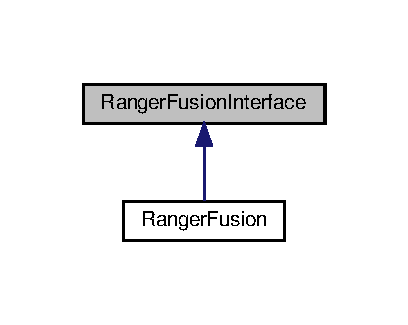
\includegraphics[width=196pt]{classRangerFusionInterface__inherit__graph}
\end{center}
\end{figure}
\subsection*{Public Member Functions}
\begin{DoxyCompactItemize}
\item 
virtual void \hyperlink{classRangerFusionInterface_ab8fdee0050521767d33179a63da91e4f}{set\+Cells} (std\+::vector$<$ \hyperlink{classCell}{Cell} $\ast$$>$ cells)=0
\begin{DoxyCompactList}\small\item\em Accepts the container of cells. \end{DoxyCompactList}\item 
\mbox{\Hypertarget{classRangerFusionInterface_ada6afdab2ce6d58a1bd0134f5e2be23f}\label{classRangerFusionInterface_ada6afdab2ce6d58a1bd0134f5e2be23f}} 
virtual void \hyperlink{classRangerFusionInterface_ada6afdab2ce6d58a1bd0134f5e2be23f}{grab\+And\+Fuse\+Data} ()=0
\begin{DoxyCompactList}\small\item\em Does two operations (1) Calls each ranger to generate data and uses this data to determine colissions with provided container of cells (2) Generates a \textquotesingle{}fusion\textquotesingle{} of the data based on collision conditions as descibed in Assignment 2 specification. \end{DoxyCompactList}\item 
virtual std\+::vector$<$ std\+::vector$<$ double $>$ $>$ \hyperlink{classRangerFusionInterface_a9d60ca5866261026b870d7c0171587f5}{get\+Raw\+Range\+Data} ()=0
\begin{DoxyCompactList}\small\item\em Returns the raw data from all sensors in the ranger container within a vector of vectors The raw data is updated every time a new fusion is requested (grab\+And\+Fuse\+Dat). The raw data is the data used for collision checking. If no fusion has occured the vector shall be empty. \end{DoxyCompactList}\item 
virtual double \hyperlink{classRangerFusionInterface_a65155605804376da4f67baf3c6f97f40}{get\+Scanning\+Area} ()=0
\begin{DoxyCompactList}\small\item\em Returns the total scanning area possible with C\+O\+NE based scanners supplied A union of all areas \href{https://en.wikipedia.org/wiki/Union_(set_theory)}{\tt https\+://en.\+wikipedia.\+org/wiki/\+Union\+\_\+(set\+\_\+theory)} \end{DoxyCompactList}\end{DoxyCompactItemize}


\subsection{Detailed Description}
Specifies the required interface for your \hyperlink{classRangerFusion}{Ranger\+Fusion} class your ranger fusion class must inherit from it. {\bfseries  You M\+U\+ST N\+OT edit this file }. 

\hyperlink{classRanger}{Ranger} Interface Class

Specifies the required interface for your \hyperlink{classRangerFusion}{Ranger\+Fusion} class your ranger fusion class must inherit from it. {\bfseries  You M\+U\+ST N\+OT edit this file }. \begin{DoxyAuthor}{Author}
Alen Alempijevic 
\end{DoxyAuthor}
\begin{DoxyVersion}{Version}
1.\+01-\/2 
\end{DoxyVersion}
\begin{DoxyDate}{Date}
2019-\/07-\/10 
\end{DoxyDate}
\begin{DoxyPrecond}{Precondition}
none 
\end{DoxyPrecond}
\begin{DoxyRefDesc}{Bug}
\item[\hyperlink{bug__bug000008}{Bug}]none reported as of 2020-\/04-\/11 \end{DoxyRefDesc}
\begin{DoxyWarning}{Warning}
students M\+U\+ST N\+OT change this class (the header file) 
\end{DoxyWarning}


\subsection{Member Function Documentation}
\mbox{\Hypertarget{classRangerFusionInterface_a9d60ca5866261026b870d7c0171587f5}\label{classRangerFusionInterface_a9d60ca5866261026b870d7c0171587f5}} 
\index{Ranger\+Fusion\+Interface@{Ranger\+Fusion\+Interface}!get\+Raw\+Range\+Data@{get\+Raw\+Range\+Data}}
\index{get\+Raw\+Range\+Data@{get\+Raw\+Range\+Data}!Ranger\+Fusion\+Interface@{Ranger\+Fusion\+Interface}}
\subsubsection{\texorpdfstring{get\+Raw\+Range\+Data()}{getRawRangeData()}}
{\footnotesize\ttfamily virtual std\+::vector$<$std\+::vector$<$double$>$ $>$ Ranger\+Fusion\+Interface\+::get\+Raw\+Range\+Data (\begin{DoxyParamCaption}{ }\end{DoxyParamCaption})\hspace{0.3cm}{\ttfamily [pure virtual]}}



Returns the raw data from all sensors in the ranger container within a vector of vectors The raw data is updated every time a new fusion is requested (grab\+And\+Fuse\+Dat). The raw data is the data used for collision checking. If no fusion has occured the vector shall be empty. 

\begin{DoxyReturn}{Returns}
std\+::vector$<$std\+::vector$<$double$>$$>$ the outer elements of the vector related to the rangers, the inner elements of vector are the respective range readings
\end{DoxyReturn}
\begin{DoxySeeAlso}{See also}
\hyperlink{classRangerFusionInterface_ada6afdab2ce6d58a1bd0134f5e2be23f}{grab\+And\+Fuse\+Data} 
\end{DoxySeeAlso}


Implemented in \hyperlink{classRangerFusion_a5780383fdffe121a7a2372a047819ba9}{Ranger\+Fusion}.

\mbox{\Hypertarget{classRangerFusionInterface_a65155605804376da4f67baf3c6f97f40}\label{classRangerFusionInterface_a65155605804376da4f67baf3c6f97f40}} 
\index{Ranger\+Fusion\+Interface@{Ranger\+Fusion\+Interface}!get\+Scanning\+Area@{get\+Scanning\+Area}}
\index{get\+Scanning\+Area@{get\+Scanning\+Area}!Ranger\+Fusion\+Interface@{Ranger\+Fusion\+Interface}}
\subsubsection{\texorpdfstring{get\+Scanning\+Area()}{getScanningArea()}}
{\footnotesize\ttfamily virtual double Ranger\+Fusion\+Interface\+::get\+Scanning\+Area (\begin{DoxyParamCaption}{ }\end{DoxyParamCaption})\hspace{0.3cm}{\ttfamily [pure virtual]}}



Returns the total scanning area possible with C\+O\+NE based scanners supplied A union of all areas \href{https://en.wikipedia.org/wiki/Union_(set_theory)}{\tt https\+://en.\+wikipedia.\+org/wiki/\+Union\+\_\+(set\+\_\+theory)} 

\begin{DoxyReturn}{Returns}
double Total area coverage
\end{DoxyReturn}
\begin{DoxySeeAlso}{See also}
\hyperlink{classRangerFusionInterface_ada6afdab2ce6d58a1bd0134f5e2be23f}{grab\+And\+Fuse\+Data} 
\end{DoxySeeAlso}


Implemented in \hyperlink{classRangerFusion_a7215e5405e808b5a853984e2b70ed6ad}{Ranger\+Fusion}.

\mbox{\Hypertarget{classRangerFusionInterface_ab8fdee0050521767d33179a63da91e4f}\label{classRangerFusionInterface_ab8fdee0050521767d33179a63da91e4f}} 
\index{Ranger\+Fusion\+Interface@{Ranger\+Fusion\+Interface}!set\+Cells@{set\+Cells}}
\index{set\+Cells@{set\+Cells}!Ranger\+Fusion\+Interface@{Ranger\+Fusion\+Interface}}
\subsubsection{\texorpdfstring{set\+Cells()}{setCells()}}
{\footnotesize\ttfamily virtual void Ranger\+Fusion\+Interface\+::set\+Cells (\begin{DoxyParamCaption}\item[{std\+::vector$<$ \hyperlink{classCell}{Cell} $\ast$$>$}]{cells }\end{DoxyParamCaption})\hspace{0.3cm}{\ttfamily [pure virtual]}}



Accepts the container of cells. 


\begin{DoxyParams}{Parameters}
{\em cells} & \\
\hline
\end{DoxyParams}


Implemented in \hyperlink{classRangerFusion_a9b69869bd1e3bca155bcecbad5ea463b}{Ranger\+Fusion}.



The documentation for this class was generated from the following file\+:\begin{DoxyCompactItemize}
\item 
rangerfusioninterface.\+h\end{DoxyCompactItemize}

\hypertarget{classRangerInterface}{}\section{Ranger\+Interface Class Reference}
\label{classRangerInterface}\index{Ranger\+Interface@{Ranger\+Interface}}


Specifies the functionality for the \hyperlink{classRanger}{Ranger} Class, your \hyperlink{classRanger}{Ranger} class must inherit from it. {\bfseries  You M\+U\+ST N\+OT edit this file }.  




{\ttfamily \#include $<$rangerinterface.\+h$>$}



Inheritance diagram for Ranger\+Interface\+:\nopagebreak
\begin{figure}[H]
\begin{center}
\leavevmode
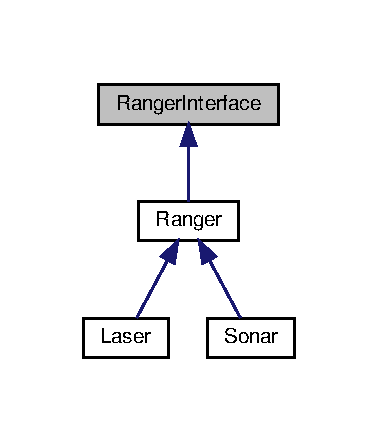
\includegraphics[width=182pt]{classRangerInterface__inherit__graph}
\end{center}
\end{figure}
\subsection*{Public Member Functions}
\begin{DoxyCompactItemize}
\item 
\mbox{\Hypertarget{classRangerInterface_a969c670cadf55a15733809116dc305c8}\label{classRangerInterface_a969c670cadf55a15733809116dc305c8}} 
virtual std\+::vector$<$ double $>$ {\bfseries generate\+Data} ()=0
\item 
virtual unsigned int \hyperlink{classRangerInterface_a37d4f89daffa8b2708dfc11034893552}{get\+Angular\+Resolution} (void)=0
\item 
virtual \hyperlink{structranger_1_1SensorPose}{ranger\+::\+Sensor\+Pose} \hyperlink{classRangerInterface_a7f6db3f603d997ad6c5aa5c7778261f4}{get\+Sensor\+Pose} (void)=0
\item 
virtual unsigned int \hyperlink{classRangerInterface_a18716da6932402b8dda75f682be6f06c}{get\+Field\+Of\+View} (void)=0
\item 
virtual double \hyperlink{classRangerInterface_a0bb29a41de5767c99081002c0590c186}{get\+Max\+Range} (void)=0
\item 
virtual double \hyperlink{classRangerInterface_ae6d501ddeeaad4a7b44d7d51ce64cb88}{get\+Min\+Range} (void)=0
\item 
virtual \hyperlink{namespaceranger_ab04465c229cc50595ffe40a891a3b135}{ranger\+::\+Sensing\+Method} \hyperlink{classRangerInterface_aeb06b9835f2b162b81917bd27797549b}{get\+Sensing\+Method} (void)=0
\item 
virtual bool \hyperlink{classRangerInterface_aecffc9bbb58379da741c18326b9e41db}{set\+Angular\+Resolution} (unsigned int resolution)=0
\item 
virtual bool \hyperlink{classRangerInterface_a452301937b5ace7ded943d8aa76a061f}{set\+Sensor\+Pose} (\hyperlink{structranger_1_1SensorPose}{ranger\+::\+Sensor\+Pose} pose)=0
\item 
virtual bool \hyperlink{classRangerInterface_a70357ca516198af45e2d503ef6af8f9f}{set\+Field\+Of\+View} (unsigned int fov)=0
\end{DoxyCompactItemize}


\subsection{Detailed Description}
Specifies the functionality for the \hyperlink{classRanger}{Ranger} Class, your \hyperlink{classRanger}{Ranger} class must inherit from it. {\bfseries  You M\+U\+ST N\+OT edit this file }. 

\subsection{Member Function Documentation}
\mbox{\Hypertarget{classRangerInterface_a37d4f89daffa8b2708dfc11034893552}\label{classRangerInterface_a37d4f89daffa8b2708dfc11034893552}} 
\index{Ranger\+Interface@{Ranger\+Interface}!get\+Angular\+Resolution@{get\+Angular\+Resolution}}
\index{get\+Angular\+Resolution@{get\+Angular\+Resolution}!Ranger\+Interface@{Ranger\+Interface}}
\subsubsection{\texorpdfstring{get\+Angular\+Resolution()}{getAngularResolution()}}
{\footnotesize\ttfamily virtual unsigned int Ranger\+Interface\+::get\+Angular\+Resolution (\begin{DoxyParamCaption}\item[{void}]{ }\end{DoxyParamCaption})\hspace{0.3cm}{\ttfamily [pure virtual]}}

Getter for Angular resolution \begin{DoxyReturn}{Returns}
angular resolution \mbox{[}deg\mbox{]} 
\end{DoxyReturn}


Implemented in \hyperlink{classRanger_a95b5013ae191d1e19b93fab002306718}{Ranger}.

\mbox{\Hypertarget{classRangerInterface_a18716da6932402b8dda75f682be6f06c}\label{classRangerInterface_a18716da6932402b8dda75f682be6f06c}} 
\index{Ranger\+Interface@{Ranger\+Interface}!get\+Field\+Of\+View@{get\+Field\+Of\+View}}
\index{get\+Field\+Of\+View@{get\+Field\+Of\+View}!Ranger\+Interface@{Ranger\+Interface}}
\subsubsection{\texorpdfstring{get\+Field\+Of\+View()}{getFieldOfView()}}
{\footnotesize\ttfamily virtual unsigned int Ranger\+Interface\+::get\+Field\+Of\+View (\begin{DoxyParamCaption}\item[{void}]{ }\end{DoxyParamCaption})\hspace{0.3cm}{\ttfamily [pure virtual]}}

Getter for field of view, for P\+O\+I\+NT based sensors F\+OV is zero \begin{DoxyReturn}{Returns}
field of view \mbox{[}deg\mbox{]} 
\end{DoxyReturn}


Implemented in \hyperlink{classRanger_a4bca7dce56b7959257d90b1f30bf0271}{Ranger}.

\mbox{\Hypertarget{classRangerInterface_a0bb29a41de5767c99081002c0590c186}\label{classRangerInterface_a0bb29a41de5767c99081002c0590c186}} 
\index{Ranger\+Interface@{Ranger\+Interface}!get\+Max\+Range@{get\+Max\+Range}}
\index{get\+Max\+Range@{get\+Max\+Range}!Ranger\+Interface@{Ranger\+Interface}}
\subsubsection{\texorpdfstring{get\+Max\+Range()}{getMaxRange()}}
{\footnotesize\ttfamily virtual double Ranger\+Interface\+::get\+Max\+Range (\begin{DoxyParamCaption}\item[{void}]{ }\end{DoxyParamCaption})\hspace{0.3cm}{\ttfamily [pure virtual]}}

Getter for maximum range \begin{DoxyReturn}{Returns}
maximum rage \mbox{[}m\mbox{]} 
\end{DoxyReturn}


Implemented in \hyperlink{classRanger_aba5e81260e55089d9ff869051156a722}{Ranger}.

\mbox{\Hypertarget{classRangerInterface_ae6d501ddeeaad4a7b44d7d51ce64cb88}\label{classRangerInterface_ae6d501ddeeaad4a7b44d7d51ce64cb88}} 
\index{Ranger\+Interface@{Ranger\+Interface}!get\+Min\+Range@{get\+Min\+Range}}
\index{get\+Min\+Range@{get\+Min\+Range}!Ranger\+Interface@{Ranger\+Interface}}
\subsubsection{\texorpdfstring{get\+Min\+Range()}{getMinRange()}}
{\footnotesize\ttfamily virtual double Ranger\+Interface\+::get\+Min\+Range (\begin{DoxyParamCaption}\item[{void}]{ }\end{DoxyParamCaption})\hspace{0.3cm}{\ttfamily [pure virtual]}}

Getter for mimimum range \begin{DoxyReturn}{Returns}
minimum rage \mbox{[}m\mbox{]} 
\end{DoxyReturn}


Implemented in \hyperlink{classRanger_a646a06d3916179b9ebc4502bad169eec}{Ranger}.

\mbox{\Hypertarget{classRangerInterface_aeb06b9835f2b162b81917bd27797549b}\label{classRangerInterface_aeb06b9835f2b162b81917bd27797549b}} 
\index{Ranger\+Interface@{Ranger\+Interface}!get\+Sensing\+Method@{get\+Sensing\+Method}}
\index{get\+Sensing\+Method@{get\+Sensing\+Method}!Ranger\+Interface@{Ranger\+Interface}}
\subsubsection{\texorpdfstring{get\+Sensing\+Method()}{getSensingMethod()}}
{\footnotesize\ttfamily virtual \hyperlink{namespaceranger_ab04465c229cc50595ffe40a891a3b135}{ranger\+::\+Sensing\+Method} Ranger\+Interface\+::get\+Sensing\+Method (\begin{DoxyParamCaption}\item[{void}]{ }\end{DoxyParamCaption})\hspace{0.3cm}{\ttfamily [pure virtual]}}

Getter for sensing method \begin{DoxyReturn}{Returns}
Sensing Method 
\end{DoxyReturn}
\begin{DoxySeeAlso}{See also}
Sensging Method 
\end{DoxySeeAlso}


Implemented in \hyperlink{classRanger_a47e30b7ec55adec5bb542278ccfee140}{Ranger}.

\mbox{\Hypertarget{classRangerInterface_a7f6db3f603d997ad6c5aa5c7778261f4}\label{classRangerInterface_a7f6db3f603d997ad6c5aa5c7778261f4}} 
\index{Ranger\+Interface@{Ranger\+Interface}!get\+Sensor\+Pose@{get\+Sensor\+Pose}}
\index{get\+Sensor\+Pose@{get\+Sensor\+Pose}!Ranger\+Interface@{Ranger\+Interface}}
\subsubsection{\texorpdfstring{get\+Sensor\+Pose()}{getSensorPose()}}
{\footnotesize\ttfamily virtual \hyperlink{structranger_1_1SensorPose}{ranger\+::\+Sensor\+Pose} Ranger\+Interface\+::get\+Sensor\+Pose (\begin{DoxyParamCaption}\item[{void}]{ }\end{DoxyParamCaption})\hspace{0.3cm}{\ttfamily [pure virtual]}}

Getter for sensor pose \begin{DoxyReturn}{Returns}
sensor pose 
\end{DoxyReturn}


Implemented in \hyperlink{classRanger_aec1e730fbf4b46b01b08f6655152fc39}{Ranger}.

\mbox{\Hypertarget{classRangerInterface_aecffc9bbb58379da741c18326b9e41db}\label{classRangerInterface_aecffc9bbb58379da741c18326b9e41db}} 
\index{Ranger\+Interface@{Ranger\+Interface}!set\+Angular\+Resolution@{set\+Angular\+Resolution}}
\index{set\+Angular\+Resolution@{set\+Angular\+Resolution}!Ranger\+Interface@{Ranger\+Interface}}
\subsubsection{\texorpdfstring{set\+Angular\+Resolution()}{setAngularResolution()}}
{\footnotesize\ttfamily virtual bool Ranger\+Interface\+::set\+Angular\+Resolution (\begin{DoxyParamCaption}\item[{unsigned int}]{resolution }\end{DoxyParamCaption})\hspace{0.3cm}{\ttfamily [pure virtual]}}

Set angular resolution method 
\begin{DoxyParams}{Parameters}
{\em resolution} & in \mbox{[}degrees\mbox{]} \\
\hline
\end{DoxyParams}
\begin{DoxyReturn}{Returns}
true if resolution supported and actioned, false is not -\/ previous setting used 
\end{DoxyReturn}


Implemented in \hyperlink{classRanger_a3dc62dcba54eefbd7a0f08cbf97d87dc}{Ranger}, and \hyperlink{classLaser_a518ac84d4631b1550330d664e161ca0a}{Laser}.

\mbox{\Hypertarget{classRangerInterface_a70357ca516198af45e2d503ef6af8f9f}\label{classRangerInterface_a70357ca516198af45e2d503ef6af8f9f}} 
\index{Ranger\+Interface@{Ranger\+Interface}!set\+Field\+Of\+View@{set\+Field\+Of\+View}}
\index{set\+Field\+Of\+View@{set\+Field\+Of\+View}!Ranger\+Interface@{Ranger\+Interface}}
\subsubsection{\texorpdfstring{set\+Field\+Of\+View()}{setFieldOfView()}}
{\footnotesize\ttfamily virtual bool Ranger\+Interface\+::set\+Field\+Of\+View (\begin{DoxyParamCaption}\item[{unsigned int}]{fov }\end{DoxyParamCaption})\hspace{0.3cm}{\ttfamily [pure virtual]}}

Set field of view 
\begin{DoxyParams}{Parameters}
{\em field} & of view \mbox{[}degrees\mbox{]} \\
\hline
\end{DoxyParams}
\begin{DoxyReturn}{Returns}
true if field of view actioned, false otherwise 
\end{DoxyReturn}


Implemented in \hyperlink{classRanger_afb5d392ca450bcce295e61c121d09157}{Ranger}, \hyperlink{classLaser_a5f140784aae7e82c2aa0f690548d6ebb}{Laser}, and \hyperlink{classSonar_a74d551d0ad61861ccf903f2535d799f0}{Sonar}.

\mbox{\Hypertarget{classRangerInterface_a452301937b5ace7ded943d8aa76a061f}\label{classRangerInterface_a452301937b5ace7ded943d8aa76a061f}} 
\index{Ranger\+Interface@{Ranger\+Interface}!set\+Sensor\+Pose@{set\+Sensor\+Pose}}
\index{set\+Sensor\+Pose@{set\+Sensor\+Pose}!Ranger\+Interface@{Ranger\+Interface}}
\subsubsection{\texorpdfstring{set\+Sensor\+Pose()}{setSensorPose()}}
{\footnotesize\ttfamily virtual bool Ranger\+Interface\+::set\+Sensor\+Pose (\begin{DoxyParamCaption}\item[{\hyperlink{structranger_1_1SensorPose}{ranger\+::\+Sensor\+Pose}}]{pose }\end{DoxyParamCaption})\hspace{0.3cm}{\ttfamily [pure virtual]}}

Set sensor pose 
\begin{DoxyParams}{Parameters}
{\em pose} & Sensor\+Pose \\
\hline
\end{DoxyParams}
\begin{DoxyReturn}{Returns}
true if offset actioned, false otherwise 
\end{DoxyReturn}


Implemented in \hyperlink{classRanger_aa55ad45d83b8c095a495677ac8873f2b}{Ranger}.



The documentation for this class was generated from the following file\+:\begin{DoxyCompactItemize}
\item 
rangerinterface.\+h\end{DoxyCompactItemize}

\hypertarget{structranger_1_1SensorPose}{}\section{ranger\+:\+:Sensor\+Pose Struct Reference}
\label{structranger_1_1SensorPose}\index{ranger\+::\+Sensor\+Pose@{ranger\+::\+Sensor\+Pose}}
\subsection*{Public Attributes}
\begin{DoxyCompactItemize}
\item 
double \hyperlink{structranger_1_1SensorPose_af3f4cc40667c93d56dd8e672c38a75e1}{x}
\item 
double \hyperlink{structranger_1_1SensorPose_ae7a4c48860c2e9f4fe7de03f8008026f}{y}
\item 
double \hyperlink{structranger_1_1SensorPose_a18751d4e746969c536714b372e3df1f6}{theta}
\end{DoxyCompactItemize}


\subsection{Member Data Documentation}
\mbox{\Hypertarget{structranger_1_1SensorPose_a18751d4e746969c536714b372e3df1f6}\label{structranger_1_1SensorPose_a18751d4e746969c536714b372e3df1f6}} 
\index{ranger\+::\+Sensor\+Pose@{ranger\+::\+Sensor\+Pose}!theta@{theta}}
\index{theta@{theta}!ranger\+::\+Sensor\+Pose@{ranger\+::\+Sensor\+Pose}}
\subsubsection{\texorpdfstring{theta}{theta}}
{\footnotesize\ttfamily double ranger\+::\+Sensor\+Pose\+::theta}

sensor angle \mbox{[}radians\mbox{]} \mbox{\Hypertarget{structranger_1_1SensorPose_af3f4cc40667c93d56dd8e672c38a75e1}\label{structranger_1_1SensorPose_af3f4cc40667c93d56dd8e672c38a75e1}} 
\index{ranger\+::\+Sensor\+Pose@{ranger\+::\+Sensor\+Pose}!x@{x}}
\index{x@{x}!ranger\+::\+Sensor\+Pose@{ranger\+::\+Sensor\+Pose}}
\subsubsection{\texorpdfstring{x}{x}}
{\footnotesize\ttfamily double ranger\+::\+Sensor\+Pose\+::x}

sensor position x axis \mbox{[}m\mbox{]} \mbox{\Hypertarget{structranger_1_1SensorPose_ae7a4c48860c2e9f4fe7de03f8008026f}\label{structranger_1_1SensorPose_ae7a4c48860c2e9f4fe7de03f8008026f}} 
\index{ranger\+::\+Sensor\+Pose@{ranger\+::\+Sensor\+Pose}!y@{y}}
\index{y@{y}!ranger\+::\+Sensor\+Pose@{ranger\+::\+Sensor\+Pose}}
\subsubsection{\texorpdfstring{y}{y}}
{\footnotesize\ttfamily double ranger\+::\+Sensor\+Pose\+::y}

sensor position y axis \mbox{[}m\mbox{]} 

The documentation for this struct was generated from the following file\+:\begin{DoxyCompactItemize}
\item 
rangerinterface.\+h\end{DoxyCompactItemize}

\hypertarget{classSonar}{}\section{Sonar Class Reference}
\label{classSonar}\index{Sonar@{Sonar}}


The \hyperlink{classSonar}{Sonar} type sensor class. This class is derived from the base class \hyperlink{classRanger}{Ranger}.  




{\ttfamily \#include $<$sonar.\+h$>$}



Inheritance diagram for Sonar\+:\nopagebreak
\begin{figure}[H]
\begin{center}
\leavevmode
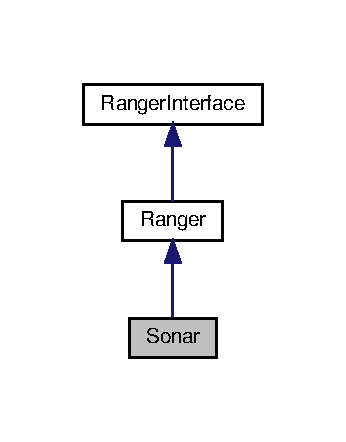
\includegraphics[width=166pt]{classSonar__inherit__graph}
\end{center}
\end{figure}


Collaboration diagram for Sonar\+:\nopagebreak
\begin{figure}[H]
\begin{center}
\leavevmode
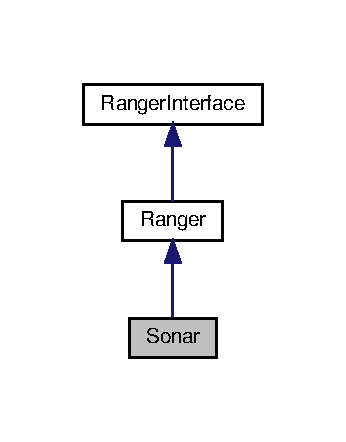
\includegraphics[width=166pt]{classSonar__coll__graph}
\end{center}
\end{figure}
\subsection*{Public Member Functions}
\begin{DoxyCompactItemize}
\item 
\hyperlink{classSonar_a71ef009d138f1e372fc35ca0cb6e85e2}{Sonar} ()
\begin{DoxyCompactList}\small\item\em \hyperlink{classSonar}{Sonar} default. \end{DoxyCompactList}\item 
\hyperlink{classSonar_a810fa5faf9ddee8ffd09c77556efda0c}{Sonar} (\hyperlink{structranger_1_1SensorPose}{ranger\+::\+Sensor\+Pose} pose)
\begin{DoxyCompactList}\small\item\em Costructor which would set defaults variables except angular resolution. \end{DoxyCompactList}\item 
\hyperlink{classSonar_ac29c8ae54d18c0ab4effbaa6fc389df4}{Sonar} (double maxr, double minr, unsigned int fov, \hyperlink{structranger_1_1SensorPose}{ranger\+::\+Sensor\+Pose} pose, \hyperlink{namespacesonar_a3fd8bcda99ebc0ba5ba1f926196fdf6b}{sonar\+::description} model)
\begin{DoxyCompactList}\small\item\em Costructor which would set all the variables of the sensor. \end{DoxyCompactList}\item 
std\+::vector$<$ double $>$ \hyperlink{classSonar_a33cc5f2df6cc1d96a59067be67eab781}{generate\+Data} ()
\begin{DoxyCompactList}\small\item\em Generates raw data for the sensor. \end{DoxyCompactList}\item 
bool \hyperlink{classSonar_a74d551d0ad61861ccf903f2535d799f0}{set\+Field\+Of\+View} (unsigned int fov)
\begin{DoxyCompactList}\small\item\em Sets the field of view (F\+OV) of the sensor based on the model. \end{DoxyCompactList}\item 
\mbox{\Hypertarget{classSonar_a8234f001a2348746880010b742ccecd2}\label{classSonar_a8234f001a2348746880010b742ccecd2}} 
void \hyperlink{classSonar_a8234f001a2348746880010b742ccecd2}{set\+Scan\+Area} ()
\begin{DoxyCompactList}\small\item\em Calculates the area that is scaned by the sensor. \end{DoxyCompactList}\item 
double \hyperlink{classSonar_ac47b8e7936dfd5c3bde262baf301d46d}{get\+Scan\+Area} ()
\begin{DoxyCompactList}\small\item\em Gets the area that is scaned by the sensor. \end{DoxyCompactList}\end{DoxyCompactItemize}
\subsection*{Additional Inherited Members}


\subsection{Detailed Description}
The \hyperlink{classSonar}{Sonar} type sensor class. This class is derived from the base class \hyperlink{classRanger}{Ranger}. 

Used for \hyperlink{classSonar}{Sonar} sensor creation 

\subsection{Constructor \& Destructor Documentation}
\mbox{\Hypertarget{classSonar_a71ef009d138f1e372fc35ca0cb6e85e2}\label{classSonar_a71ef009d138f1e372fc35ca0cb6e85e2}} 
\index{Sonar@{Sonar}!Sonar@{Sonar}}
\index{Sonar@{Sonar}!Sonar@{Sonar}}
\subsubsection{\texorpdfstring{Sonar()}{Sonar()}\hspace{0.1cm}{\footnotesize\ttfamily [1/3]}}
{\footnotesize\ttfamily Sonar\+::\+Sonar (\begin{DoxyParamCaption}{ }\end{DoxyParamCaption})}



\hyperlink{classSonar}{Sonar} default. 

max range\+: 10 min range\+: 0.\+2 fov\+: 20 position\+: 0,0,0 model\+:S\+N-\/001 \mbox{\Hypertarget{classSonar_a810fa5faf9ddee8ffd09c77556efda0c}\label{classSonar_a810fa5faf9ddee8ffd09c77556efda0c}} 
\index{Sonar@{Sonar}!Sonar@{Sonar}}
\index{Sonar@{Sonar}!Sonar@{Sonar}}
\subsubsection{\texorpdfstring{Sonar()}{Sonar()}\hspace{0.1cm}{\footnotesize\ttfamily [2/3]}}
{\footnotesize\ttfamily Sonar\+::\+Sonar (\begin{DoxyParamCaption}\item[{\hyperlink{structranger_1_1SensorPose}{ranger\+::\+Sensor\+Pose}}]{pose }\end{DoxyParamCaption})}



Costructor which would set defaults variables except angular resolution. 


\begin{DoxyParams}{Parameters}
{\em pose} & position \{x,y,theta\} \\
\hline
\end{DoxyParams}
\mbox{\Hypertarget{classSonar_ac29c8ae54d18c0ab4effbaa6fc389df4}\label{classSonar_ac29c8ae54d18c0ab4effbaa6fc389df4}} 
\index{Sonar@{Sonar}!Sonar@{Sonar}}
\index{Sonar@{Sonar}!Sonar@{Sonar}}
\subsubsection{\texorpdfstring{Sonar()}{Sonar()}\hspace{0.1cm}{\footnotesize\ttfamily [3/3]}}
{\footnotesize\ttfamily Sonar\+::\+Sonar (\begin{DoxyParamCaption}\item[{double}]{maxr,  }\item[{double}]{minr,  }\item[{unsigned int}]{fov,  }\item[{\hyperlink{structranger_1_1SensorPose}{ranger\+::\+Sensor\+Pose}}]{pose,  }\item[{\hyperlink{namespacesonar_a3fd8bcda99ebc0ba5ba1f926196fdf6b}{sonar\+::description}}]{model }\end{DoxyParamCaption})}



Costructor which would set all the variables of the sensor. 


\begin{DoxyParams}{Parameters}
{\em maximum} & range \\
\hline
{\em minimum} & range \\
\hline
{\em angular} & resolution \\
\hline
{\em F\+OV} & -\/ angle \mbox{[}deg\mbox{]} \\
\hline
{\em position} & x \mbox{[}m\mbox{]}, y \mbox{[}m\mbox{]}, angle \mbox{[}radians\mbox{]} \\
\hline
\end{DoxyParams}


\subsection{Member Function Documentation}
\mbox{\Hypertarget{classSonar_a33cc5f2df6cc1d96a59067be67eab781}\label{classSonar_a33cc5f2df6cc1d96a59067be67eab781}} 
\index{Sonar@{Sonar}!generate\+Data@{generate\+Data}}
\index{generate\+Data@{generate\+Data}!Sonar@{Sonar}}
\subsubsection{\texorpdfstring{generate\+Data()}{generateData()}}
{\footnotesize\ttfamily std\+::vector$<$ double $>$ Sonar\+::generate\+Data (\begin{DoxyParamCaption}{ }\end{DoxyParamCaption})\hspace{0.3cm}{\ttfamily [virtual]}}



Generates raw data for the sensor. 

\begin{DoxyReturn}{Returns}
vector containing senor data
\end{DoxyReturn}
Data from the sensor is just 1 distance measurement. 

Implements \hyperlink{classRanger_a1ac4a84f251b0793fc262643080f084a}{Ranger}.

\mbox{\Hypertarget{classSonar_ac47b8e7936dfd5c3bde262baf301d46d}\label{classSonar_ac47b8e7936dfd5c3bde262baf301d46d}} 
\index{Sonar@{Sonar}!get\+Scan\+Area@{get\+Scan\+Area}}
\index{get\+Scan\+Area@{get\+Scan\+Area}!Sonar@{Sonar}}
\subsubsection{\texorpdfstring{get\+Scan\+Area()}{getScanArea()}}
{\footnotesize\ttfamily double Sonar\+::get\+Scan\+Area (\begin{DoxyParamCaption}{ }\end{DoxyParamCaption})}



Gets the area that is scaned by the sensor. 

Calculates the area scanned by the sonar as a circle sector (pizza slice). \mbox{\Hypertarget{classSonar_a74d551d0ad61861ccf903f2535d799f0}\label{classSonar_a74d551d0ad61861ccf903f2535d799f0}} 
\index{Sonar@{Sonar}!set\+Field\+Of\+View@{set\+Field\+Of\+View}}
\index{set\+Field\+Of\+View@{set\+Field\+Of\+View}!Sonar@{Sonar}}
\subsubsection{\texorpdfstring{set\+Field\+Of\+View()}{setFieldOfView()}}
{\footnotesize\ttfamily bool Sonar\+::set\+Field\+Of\+View (\begin{DoxyParamCaption}\item[{unsigned int}]{fov }\end{DoxyParamCaption})\hspace{0.3cm}{\ttfamily [virtual]}}



Sets the field of view (F\+OV) of the sensor based on the model. 


\begin{DoxyParams}{Parameters}
{\em F\+OV} & value \mbox{[}deg\mbox{]} \\
\hline
\end{DoxyParams}
\begin{DoxyReturn}{Returns}
True if actioned, false otherwise
\end{DoxyReturn}
F\+OV would be a value between 0 and 360 degrees for the command to be actioned if supported (only 20 is supported by S\+N-\/001) 

Reimplemented from \hyperlink{classRanger_afb5d392ca450bcce295e61c121d09157}{Ranger}.



The documentation for this class was generated from the following files\+:\begin{DoxyCompactItemize}
\item 
sonar.\+h\item 
sonar.\+cpp\end{DoxyCompactItemize}

\hypertarget{structfusionGeometry_1_1sonarScan}{}\section{fusion\+Geometry\+:\+:sonar\+Scan Struct Reference}
\label{structfusionGeometry_1_1sonarScan}\index{fusion\+Geometry\+::sonar\+Scan@{fusion\+Geometry\+::sonar\+Scan}}


{\ttfamily \#include $<$rangerfusion.\+h$>$}



Collaboration diagram for fusion\+Geometry\+:\+:sonar\+Scan\+:\nopagebreak
\begin{figure}[H]
\begin{center}
\leavevmode
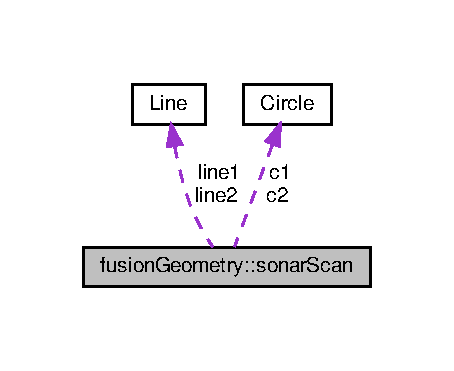
\includegraphics[width=218pt]{structfusionGeometry_1_1sonarScan__coll__graph}
\end{center}
\end{figure}
\subsection*{Public Attributes}
\begin{DoxyCompactItemize}
\item 
\hyperlink{classLine}{Line} \hyperlink{structfusionGeometry_1_1sonarScan_a5f7f2a2cbf85f169c286d2ec1455e3c8}{line1}
\item 
\hyperlink{classLine}{Line} \hyperlink{structfusionGeometry_1_1sonarScan_afb325a62186cf1333025c6bcda04bb36}{line2}
\item 
\hyperlink{classCircle}{Circle} \hyperlink{structfusionGeometry_1_1sonarScan_a21c1254ebacf46d3f3052469417534e9}{c1}
\item 
\hyperlink{classCircle}{Circle} \hyperlink{structfusionGeometry_1_1sonarScan_a6ad2411596ebd31d89123affef6930c7}{c2}
\end{DoxyCompactItemize}


\subsection{Detailed Description}
Structure for a sonar scan 

\subsection{Member Data Documentation}
\mbox{\Hypertarget{structfusionGeometry_1_1sonarScan_a21c1254ebacf46d3f3052469417534e9}\label{structfusionGeometry_1_1sonarScan_a21c1254ebacf46d3f3052469417534e9}} 
\index{fusion\+Geometry\+::sonar\+Scan@{fusion\+Geometry\+::sonar\+Scan}!c1@{c1}}
\index{c1@{c1}!fusion\+Geometry\+::sonar\+Scan@{fusion\+Geometry\+::sonar\+Scan}}
\subsubsection{\texorpdfstring{c1}{c1}}
{\footnotesize\ttfamily \hyperlink{classCircle}{Circle} fusion\+Geometry\+::sonar\+Scan\+::c1}

Min range \mbox{\Hypertarget{structfusionGeometry_1_1sonarScan_a6ad2411596ebd31d89123affef6930c7}\label{structfusionGeometry_1_1sonarScan_a6ad2411596ebd31d89123affef6930c7}} 
\index{fusion\+Geometry\+::sonar\+Scan@{fusion\+Geometry\+::sonar\+Scan}!c2@{c2}}
\index{c2@{c2}!fusion\+Geometry\+::sonar\+Scan@{fusion\+Geometry\+::sonar\+Scan}}
\subsubsection{\texorpdfstring{c2}{c2}}
{\footnotesize\ttfamily \hyperlink{classCircle}{Circle} fusion\+Geometry\+::sonar\+Scan\+::c2}

data point distance \mbox{\Hypertarget{structfusionGeometry_1_1sonarScan_a5f7f2a2cbf85f169c286d2ec1455e3c8}\label{structfusionGeometry_1_1sonarScan_a5f7f2a2cbf85f169c286d2ec1455e3c8}} 
\index{fusion\+Geometry\+::sonar\+Scan@{fusion\+Geometry\+::sonar\+Scan}!line1@{line1}}
\index{line1@{line1}!fusion\+Geometry\+::sonar\+Scan@{fusion\+Geometry\+::sonar\+Scan}}
\subsubsection{\texorpdfstring{line1}{line1}}
{\footnotesize\ttfamily \hyperlink{classLine}{Line} fusion\+Geometry\+::sonar\+Scan\+::line1}

left line \mbox{\Hypertarget{structfusionGeometry_1_1sonarScan_afb325a62186cf1333025c6bcda04bb36}\label{structfusionGeometry_1_1sonarScan_afb325a62186cf1333025c6bcda04bb36}} 
\index{fusion\+Geometry\+::sonar\+Scan@{fusion\+Geometry\+::sonar\+Scan}!line2@{line2}}
\index{line2@{line2}!fusion\+Geometry\+::sonar\+Scan@{fusion\+Geometry\+::sonar\+Scan}}
\subsubsection{\texorpdfstring{line2}{line2}}
{\footnotesize\ttfamily \hyperlink{classLine}{Line} fusion\+Geometry\+::sonar\+Scan\+::line2}

right line 

The documentation for this struct was generated from the following file\+:\begin{DoxyCompactItemize}
\item 
rangerfusion.\+h\end{DoxyCompactItemize}

%--- End generated contents ---

% Index
\backmatter
\newpage
\phantomsection
\clearemptydoublepage
\addcontentsline{toc}{chapter}{Index}
\printindex

\end{document}
